\section{Overview}
\label{sec:overview}

\begin{figure}[H]
    \centering
    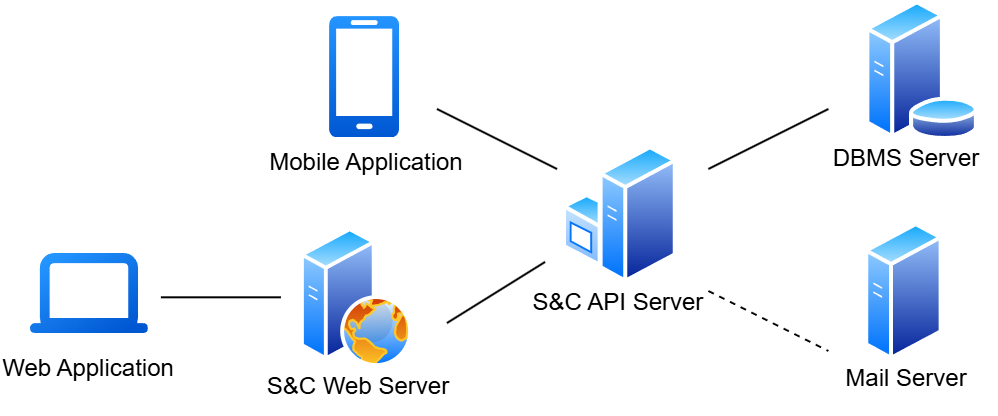
\includegraphics[width=0.9\linewidth]{Images/Architecture design/architecture.png}
    \caption{S\&C architecture overview}
    \label{fig:enter-label}
\end{figure}

The S\&C system is designed using a layered client-server architecture. The system is structured into distinct components, each responsible for specific functionalities such as user management, internship matching, notification handling, and feedback processing. Communication between these components is facilitated through RESTful APIs. This architecture ensures modularity, scalability, and ease of maintenance, allowing for efficient handling of user interactions and system operations.

Client side: 
\begin{itemize}
    \item \textbf{Web Application}: serves as the primary user interface for accessing the S\&C platform. It allows all users (students, companies, and universities) to connect to the system and perform essential operations such as registration, login, and profile management. Through the WebApp, students can search for available internships, apply for them, and track the status of their applications and active internship. Companies can create, update, and manage internship offers, while universities can monitor internship statuses and handle complaints or issues raised during internship. The platform also allows users to create or modify their profiles, including CVs and skills, and manage preferences for internship notifications. The WebApp is designed to be responsive and accessible from any modern browser, offering a smooth experience on both desktop and mobile devices.
    \item \textbf{Mobile Application}: provides a dedicated and optimized version of the S\&C platform for mobile users. It is designed to offer a seamless and intuitive experience for users on the go. Students can easily search for and apply to internships, receive push notifications about new internship offers or application updates, and monitor the status of their applications. Companies can also use the mobile application to create and manage internship offers; however, for tasks that require detailed data entry or management, the desktop version is more convenient and suitable for their needs. In contrast, the mobile application is primarily designed for students who require quick access to the platform’s functionalities. The mobile app supports real-time notifications and is available on both iOS and Android, ensuring accessibility and connectivity for all users.
\end{itemize}
Server side:
\begin{itemize}
    \item \textbf{Web Server}: manages communication with users by receiving and processing their requests. It acts as the gateway between the user and the system, ensuring that all incoming requests are appropriately handled. Additionally, it performs load balancing, distributing incoming traffic across multiple replicas of the S\&C Server to ensure scalability and high availability. The Web Server also handles user sessions, ensuring that users' activities are properly tracked and maintained throughout their interaction with the platform.
    \item \textbf{S\&C API Server}:  is the core component of the system, responsible for processing all requests and managing the primary business functionalities. It hosts the components that handle specific tasks such as user management, internship offers, matchmaking, notifications, and feedback processing. The server acts as the central point of communication between the client applications and the DBMS. All client requests (from the WebApp and Mobile Application) are routed to the appropriate component through a centralized API Gateway, which manages request routing, authentication, and load balancing. To ensure reliability, scalability, and high availability, this Server is deployed across multiple machines or containers. Communication between components can be handled via RESTful APIs for synchronous operations or message brokers (e.g., Apache Kafka) for asynchronous tasks.
    \item \textbf{DBMS Server}: stores all persistent data related to users, students, companies, internships, and interactions within the system. It acts as the primary repository for critical system information, including user profiles, internship offers, applications, feedback, and complaints. The DBMS Server is designed for data integrity, consistency, and quick retrieval of large datasets. It is optimized for performance and supports complex queries needed for matchmaking, reporting, and analytics.
\end{itemize}

\section{Component View}
\label{sec:component_view}
This section presents a detailed breakdown of the components in the system, including their responsibilities, interfaces, and interactions.

\subsection{Component Diagram}
\label{sec:component_diagram}
\begin{figure}[H]
    \centering
    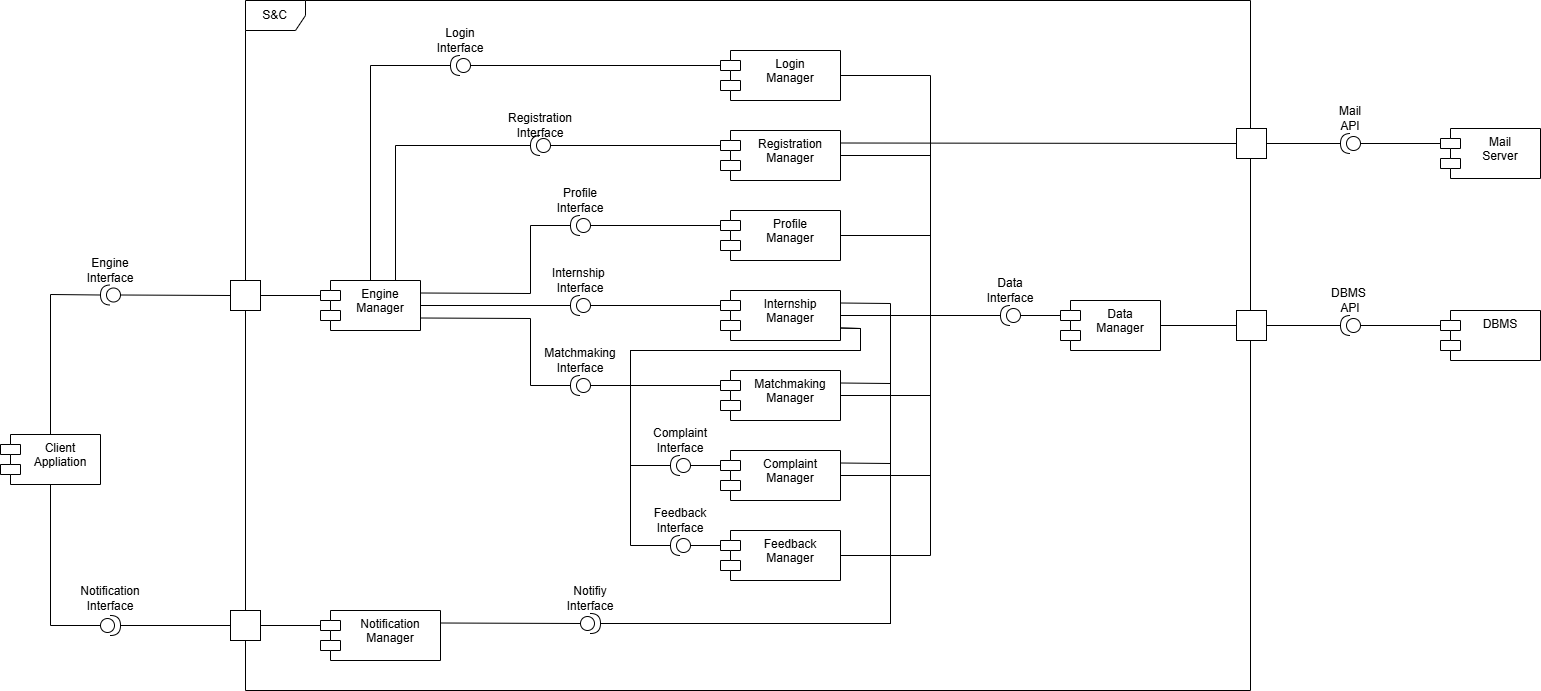
\includegraphics[width=1\linewidth]{Images/Component diagrams/ComponentDiagram.png}
    \caption{S\&C component diagram }
    \label{fig:enter-label}
\end{figure}

\subsection{Components Description}
\label{sec:component_diagram}
The components are:
\begin{itemize}
    \item \textbf{Client Application}: is the central access point for users to interact with the system. It provides the user interface through which users can perform key actions, such as logging into their accounts, registering as new users, managing personal information, submitting feedback, and accessing internship opportunities. The Client Application acts as the bridge between the user and the underlying services, sending requests to appropriate components and receiving responses to display the necessary information to the user.
    \item \textbf{Engine Manager}: serves as the core orchestration component within the system. It receives and processes user requests originating from the Client Application and coordinates the execution of these tasks by delegating them to appropriate services, such as the Login Manager, Internship Manager, or Notification Manager. By managing inter-component communication, the Engine Manager ensures the system operates efficiently and cohesively.
    \item \textbf{Login Manager}: handles the entire user authentication process. It verifies credentials provided during the login attempt by querying the DBMS to check for valid user data. If the credentials match, the Login Manager grants access to the system, ensuring that only authorized users can interact with protected services. It also manages failed login attempts, providing appropriate feedback to the user.

    \begin{figure}[H]
        \centering
        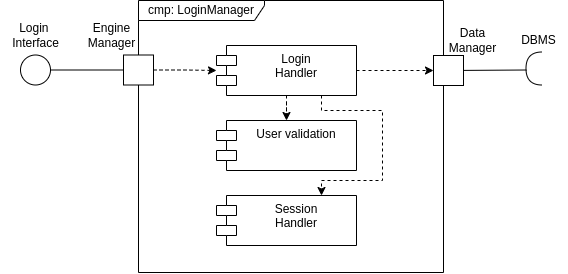
\includegraphics[width=0.9\linewidth]{Images/Component diagrams/ComponentDiagram_Login.png}
        \caption{Login manager component diagram}
        \label{fig:enter-label}
    \end{figure}
    
    \item \textbf{Registration Manager}: oversees the user registration process, enabling new users to create accounts within the system. It validates user-provided input (e.g., name, email, password) and securely communicates with the DBMS to store new account details. Additionally, it can trigger email confirmations through the Mail Server to verify user identities and ensure secure onboarding.

    \begin{figure}[H]
        \centering
        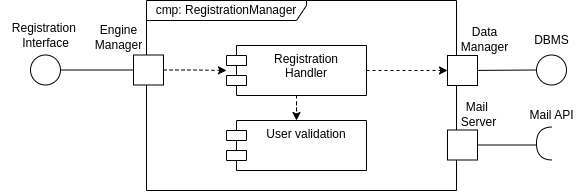
\includegraphics[width=0.9\linewidth]{Images/Component diagrams/ComponentDiagram_Registration.png}
        \caption{Registration manager component diagram}
        \label{fig:enter-label}
    \end{figure}
    
    \item \textbf{Profile Manager}: is responsible for handling all operations related to user profiles. It allows users to retrieve, view, and update personal data such as contact details, resumes, or preferences. This component ensures the integrity of profile updates by interacting directly with the DBMS to persist changes. It acts as a crucial service for maintaining user data consistency across the platform.

    \begin{figure}[H]
        \centering
        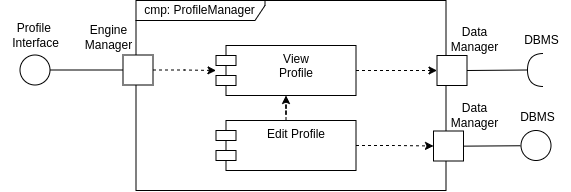
\includegraphics[width=0.9\linewidth]{Images/Component diagrams/ComponentDiagram_Profile.png}
        \caption{Profile manager component diagram}
        \label{fig:enter-label}
    \end{figure}
    
    \item \textbf{Internship Manager}: manages all operations related to internship opportunities. It allows system administrators to create, update, and delete internship postings while enabling users to search for and apply to available positions. It interacts with the DBMS to persist internship data, including details like job descriptions, requirements, and application deadlines. This service ensures up-to-date internship information is always available to users.

    \begin{figure}[H]
        \centering
        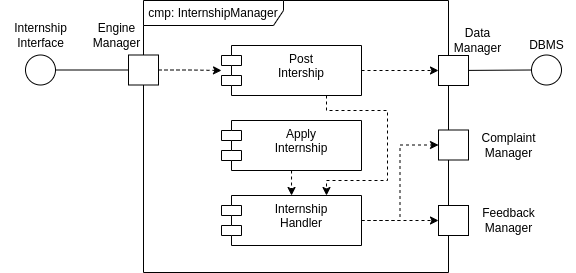
\includegraphics[width=0.9\linewidth]{Images/Component diagrams/ComponentDiagram_Internship.png}
        \caption{Internship manager component diagram}
        \label{fig:enter-label}
    \end{figure}
    
    \item \textbf{Matchmaking Manager}: is a specialized component that aligns user profiles with suitable internship opportunities. It leverages user data—such as resumes, preferences, and skills—and compares it with internship requirements stored in the DBMS. By running matching algorithms, it identifies relevant opportunities for users and generates recommendations, streamlining the search process for internships.
    \item \textbf{Complaint Manager}: allows users to report issues, concerns, or grievances within the system. It provides a structured mechanism to log complaints, which are stored in the DBMS for review and resolution by administrators. The Complaint Manager ensures that user-reported problems are tracked and appropriately addressed to improve overall user satisfaction.

    \begin{figure}[H]
        \centering
        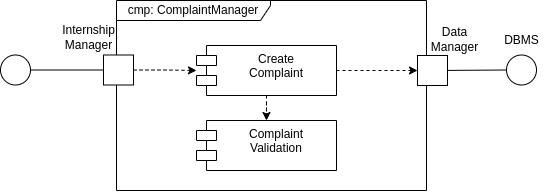
\includegraphics[width=0.9\linewidth]{Images/Component diagrams/ComponentDiagram_Complaint.png}
        \caption{Complaint manager component diagram}
        \label{fig:enter-label}
    \end{figure}
    
    \item \textbf{Feedback Manager}: is responsible for collecting and managing feedback submitted by users. It allows users to share their experiences or provide evaluations of system services. The component interacts with the DBMS to store feedback, which can later be analyzed to identify areas for improvement. This ensures continuous enhancement of the system based on user input.

    \begin{figure}[H]
        \centering
        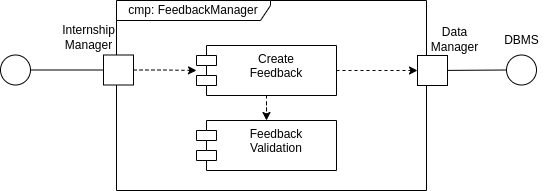
\includegraphics[width=0.9\linewidth]{Images/Component diagrams/ComponentDiagram_Feedback.png}
        \caption{Feedback manager component diagram}
        \label{fig:enter-label}
    \end{figure}
    
    \item \textbf{Notification Manager}: handles the delivery of system notifications to users. It processes requests from other components, such as the Engine Manager or Complaint Manager, to notify users about updates, events, or critical actions requiring attention. Notifications can be sent via in-app messages or through integration with the Mail Server for email delivery. This component ensures users remain up to date with relevant information.
    \item \textbf{Data Manager}: acts as the intermediary layer responsible for managing communication between components and the DBMS. It handles data retrieval, insertion, and updates, ensuring that services have seamless access to accurate and consistent data. The Data Manager ensures the integrity and security of the system’s database operations, facilitating efficient data management.
    \item \textbf{DBMS}: serves as the centralized data repository for the system. It stores all essential information, including user credentials, profiles, internship postings, complaints, and feedback. The DBMS ensures data persistence, consistency, and availability, enabling components to query and update data as needed. It forms the backbone of the system's data management architecture.
\end{itemize}

% Add the description of each component here.

\section{Deployment View}
\label{sec:deployment_view}
The deployment view describes how the system is physically deployed and the interactions between its components.
\begin{figure}[H]
    \centering
    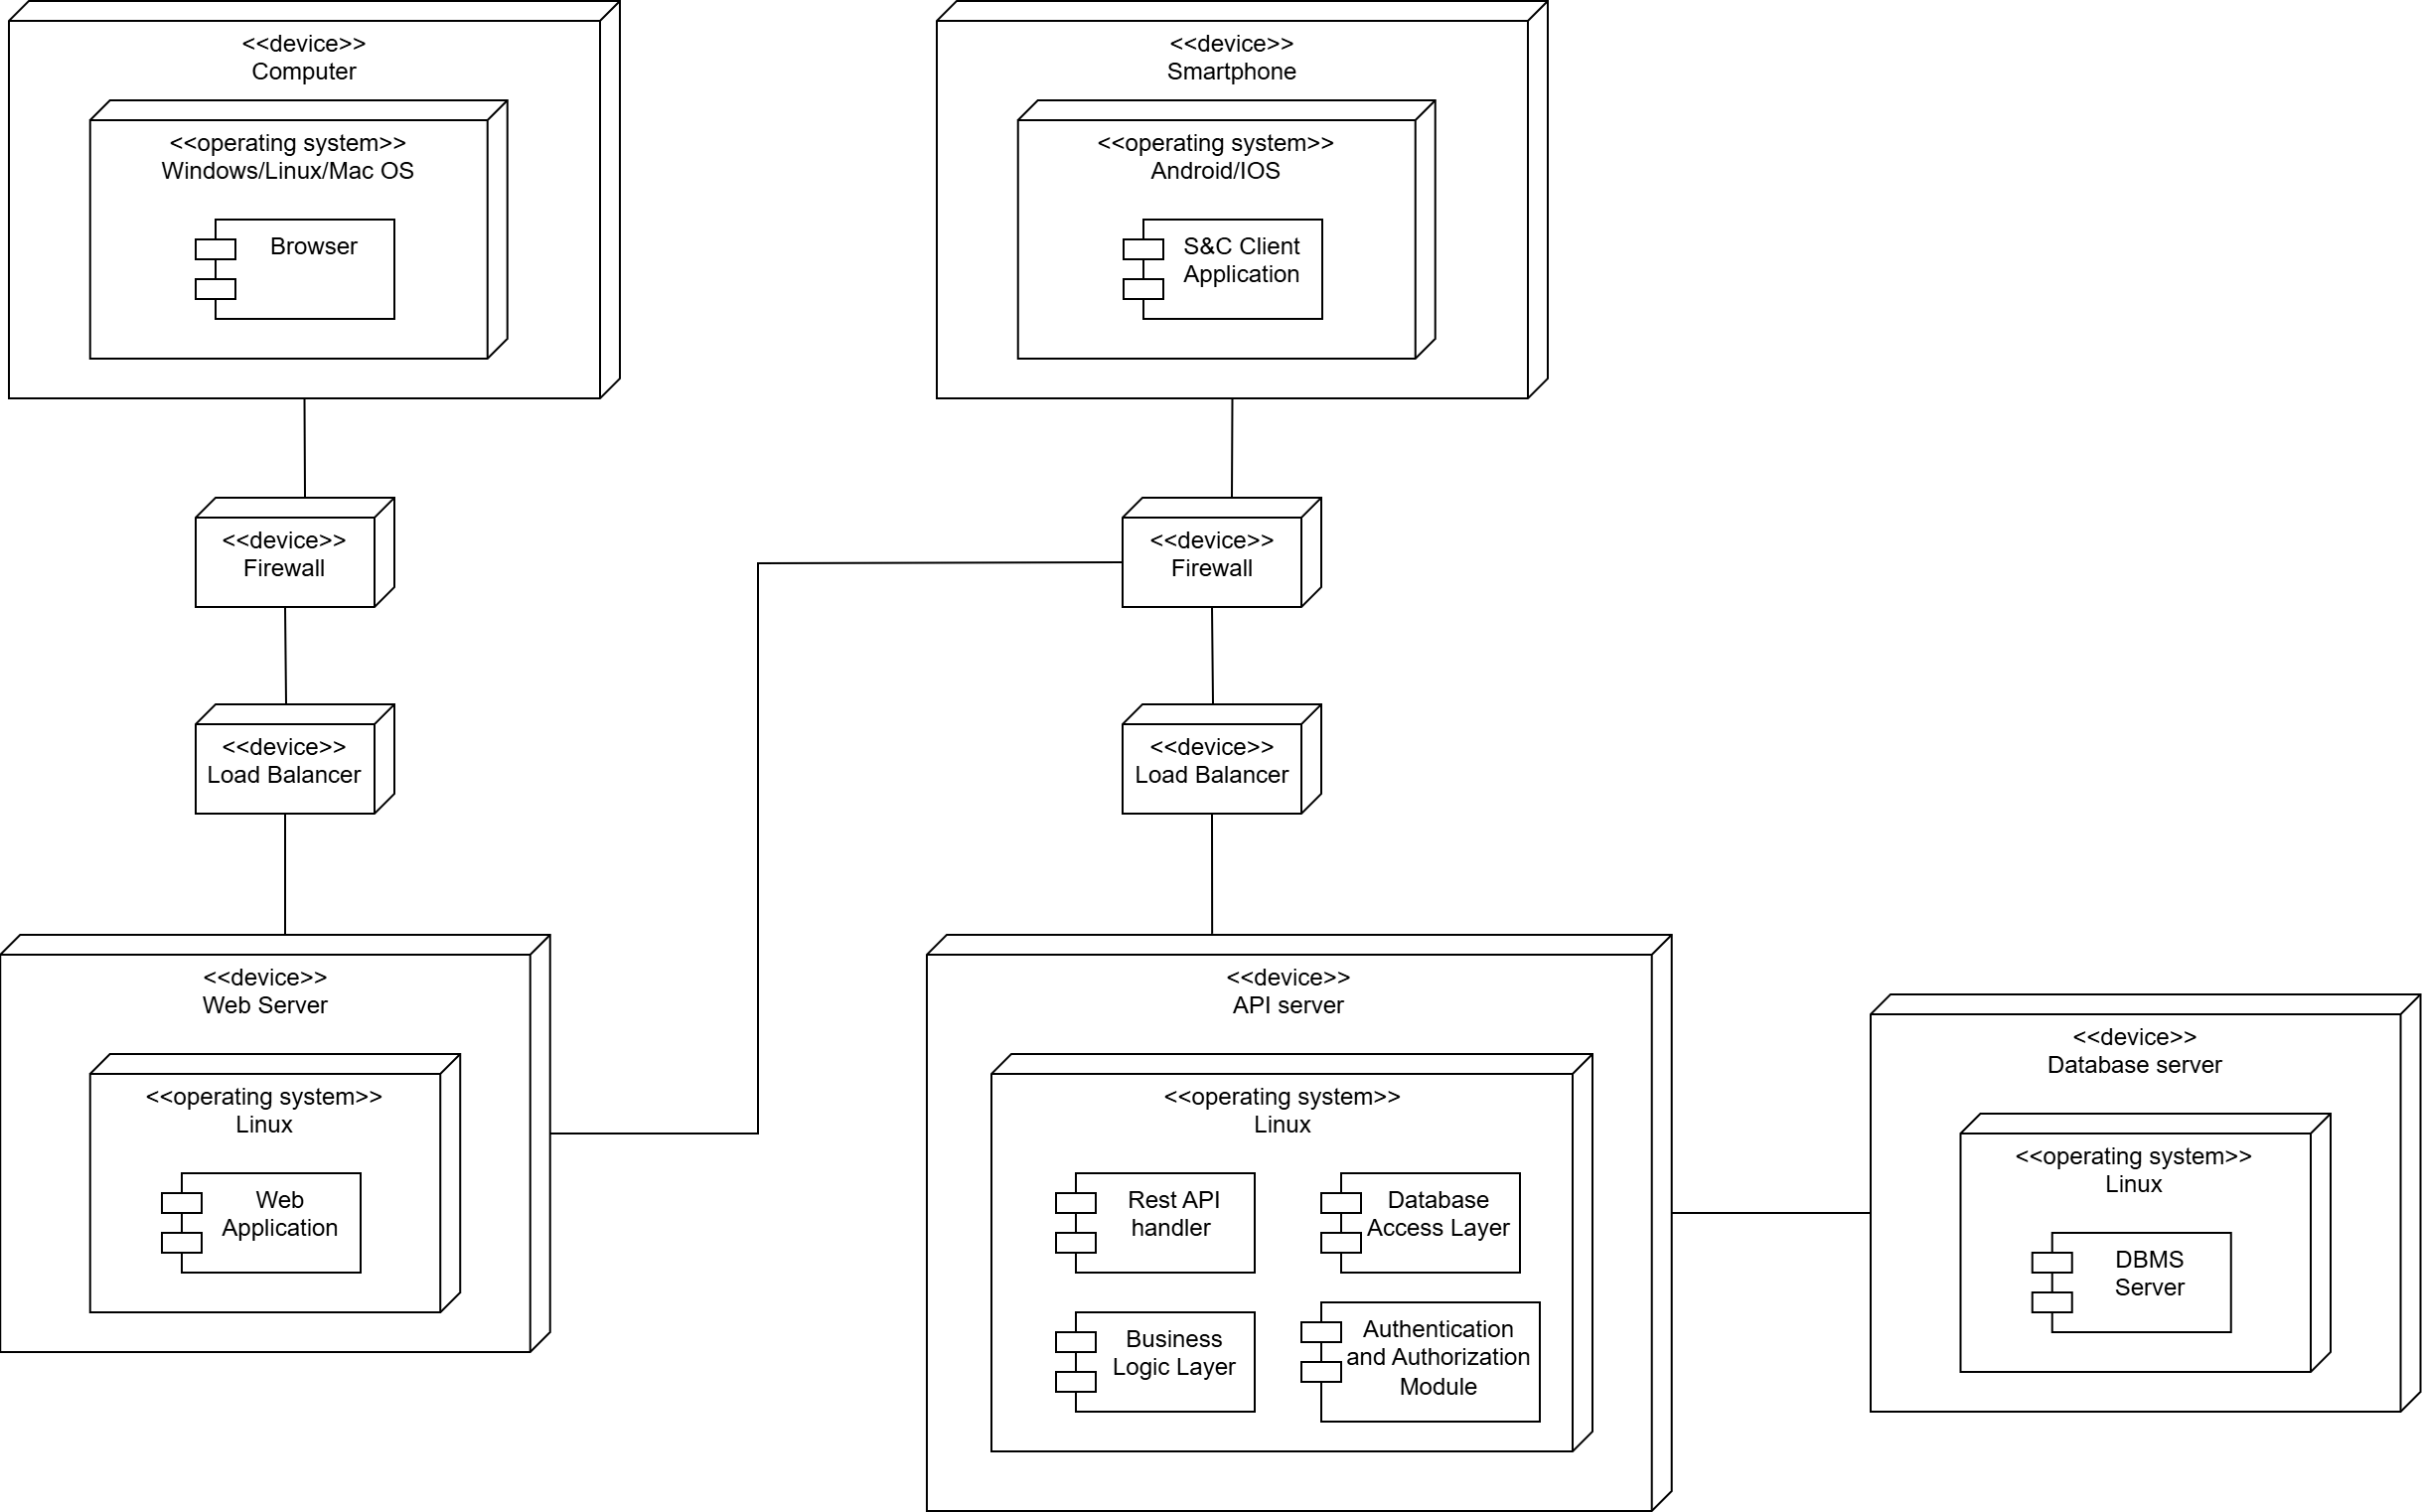
\includegraphics[width=1\linewidth]{Images/Deployment diagram/deploymentView.png}
    \caption{Deployment view diagram}
    \label{fig:enter-label}
\end{figure}

\textbf{Client Devices} \\
The system supports two types of client devices:
\begin{itemize}
    \item Computers: users can access the system via browsers on devices running different operating systems. The browser-based interface ensures cross-platform compatibility and ease of access.
    \item Smartphones: Users on Android or iOS can interact with the system through a dedicated S\&C Client Application, offering a mobile-friendly experience with tailored functionalities.
\end{itemize}

\textbf{Firewall} \\
The communication between the client devices and the backbend system is safeguarded by a Firewall. It filters incoming and outgoing traffic, protecting the system from unauthorized access, malicious attacks and data breaches.

\textbf{Load Balancer} \\
The Load Balancer is used to maintain system availability and performance by distributing incoming request across multiple backend servers. This ensures that non single server becomes a bottleneck, improving reliability and accommodating high traffic volumes.

\textbf{Web Server} \\
It serves as the entry point for users interacting via browser. It hosts the Web Application which handles the frontend functionality, rendering the user interface and responding to user actions and session management, maintaining session continuity for user logged in via web browsers.
\textbf{API Server} \\
The S\&C API Server is the heart of the system's backend logic. It is composed by several key components:
\begin{itemize}
    \item Rest API Handler: acts as the communication bridge between client requests and backend logic, ensuring proper routing and handling of API calls.
    \item Business Logic Layer: implements the core system functionalities such as processing user actions, handling workflows and executing business rules.
    \item Database Access Layer: provides a secure and optimized interface for querying and updating data in the database server.
    \item Authentication and Authorization Module: enforces user authentication and role-based permissiones to protect sensistive operations and data.
\end{itemize}

\textbf{Database server} \\
The Database server manages the system's data using a DBMS.

\section{Runtime View}
\label{sec:runtime_view}
In this section, S\&C system are presented through sequence diagrams. Initially, the actions of the S\&C system are shown from the perspective of the student user, such as logging in, applying for internships, updating their profile, and managing their preferences. Then, the actions are presented from the perspective of the company user, which involve more business-oriented functionalities, such as managing internship offers, reviewing applications, and scheduling interviews. Finally, university ones, such as the internship interruption.

\newcounter{uc}
\setcounter{uc}{1}
\newcommand{\cuc}{\theuc\stepcounter{uc}}

\textbf{UC\cuc\  - User registration} \\
The figure shows the registration process for students and companies. Once the request is sent it will automatically start the process of authentication which is managed by the Registration manager. The process continues with the student/company filling in the necessary information in order to successfully create the users profile. As soon as the form is submitted and sent to the registration manager, the database is checked to control whether another user with the same information already exists on the platform. If there is no user with the same credentials then a new user is created and added to the corresponding table.
\begin{center}
    \begin{figure}[H]
        \centering
        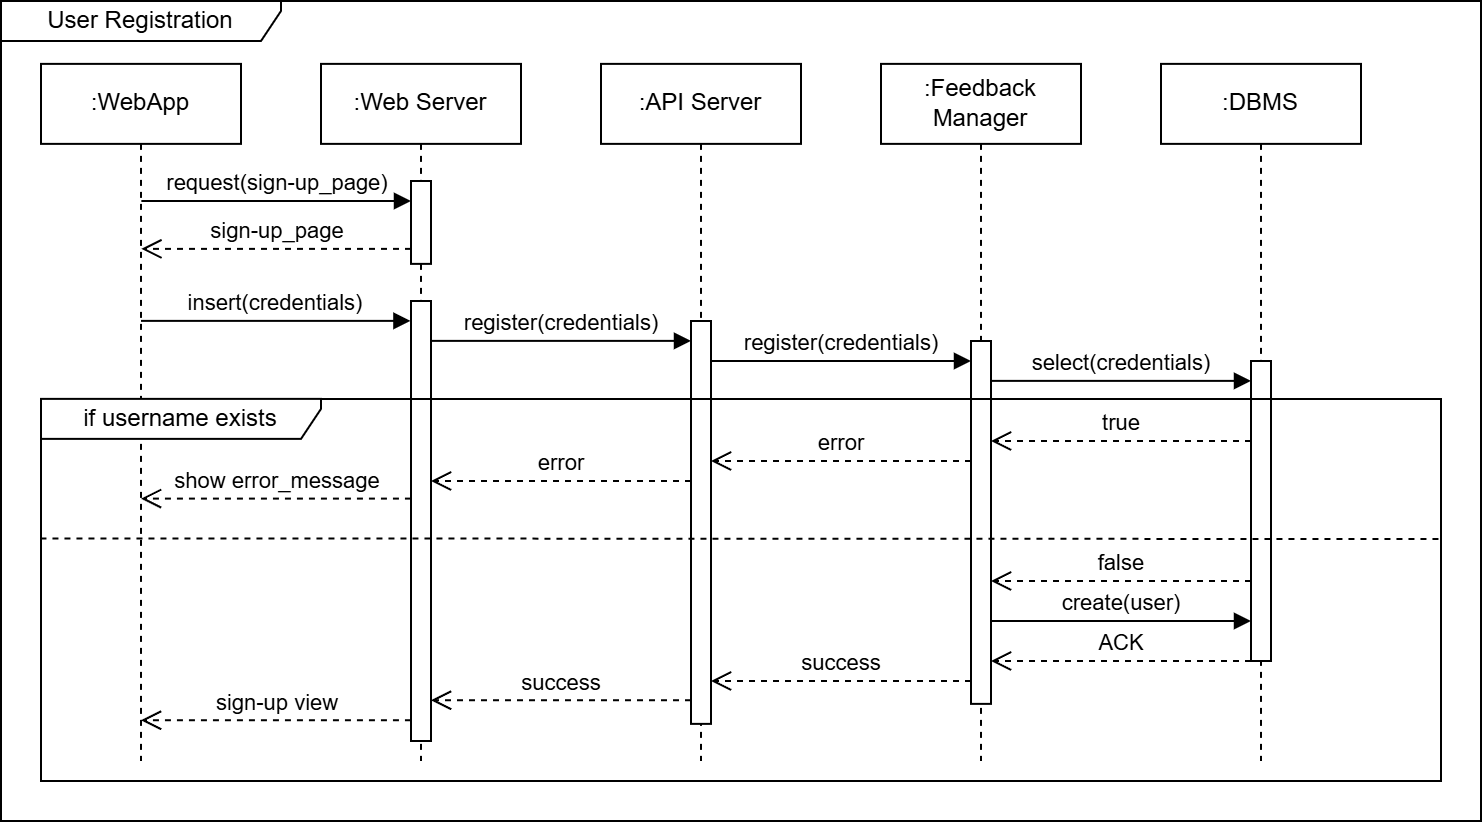
\includegraphics[width=1\linewidth]{Images/Sequence diagrams/UC1.png}
        \caption{Student Registration}
        \label{fig:enter-label}
    \end{figure}
\end{center}

\textbf{UC\cuc\  - User, student, company or university login} \\
The figure shows the process of a user login. Even if the information of every user has been stored in a separate database, one for each type of user, the process is the same.
\begin{center}
    \begin{figure}[H]
        \centering
        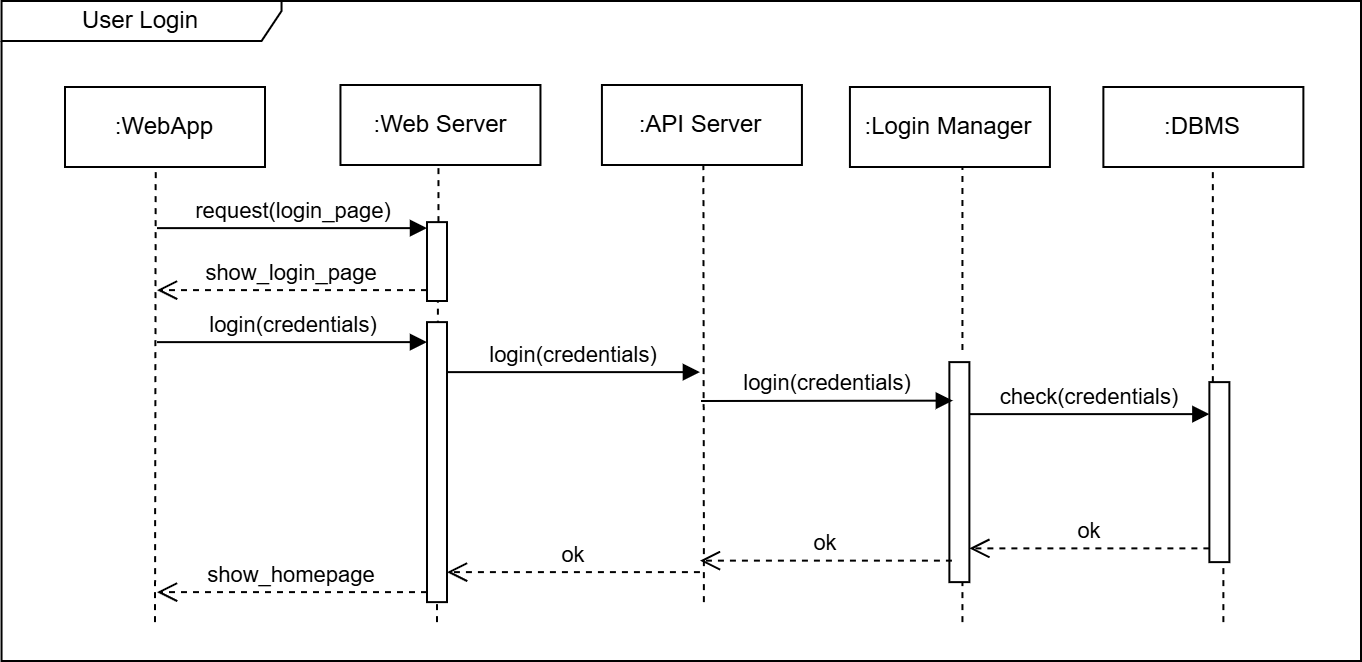
\includegraphics[width=1\linewidth]{Images/Sequence diagrams/UC2.png}
        \caption{User Login}
        \label{fig:enter-label}
    \end{figure}
\end{center}
    

\textbf{UC\cuc\  - Student’s account activation} \\
The figure shows the process of upgrading an account from standard registered user to a verified students account. After inserting the additional details required to do the upgrade correctly and after checking that there are no other students with the same credentials the Notification manager proceeds to send an email containing a verification link that the student must press in order to confirm the upgrade.
\begin{center}
    \begin{figure}[H]
        \centering
        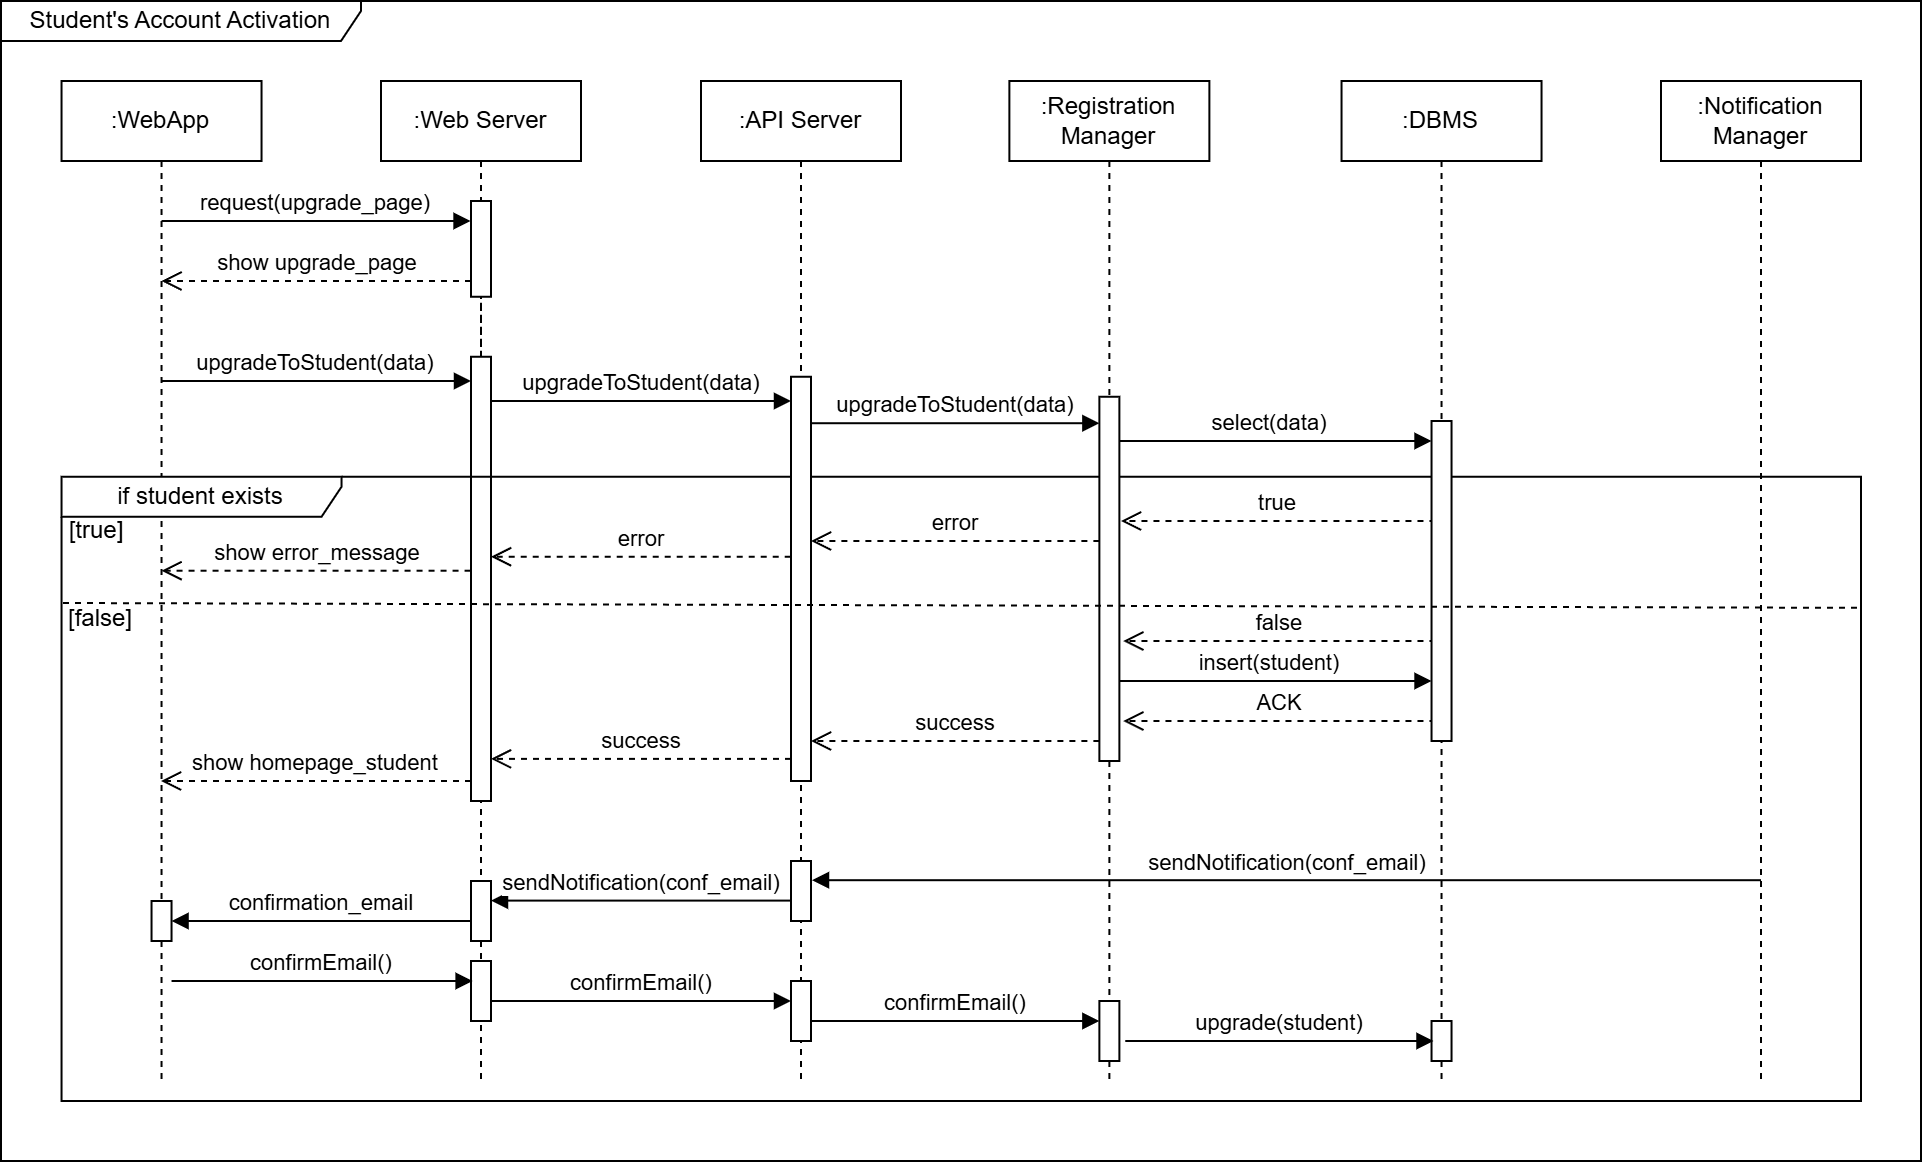
\includegraphics[width=1\linewidth]{Images/Sequence diagrams/UC3.png}
        \caption{Student's Account Activation}
        \label{fig:enter-label}
    \end{figure}
\end{center}


\textbf{UC\cuc\  - Student modifies their profile or updates their CV} \\
The diagram outlines the process for updating a student's profile. The WebApp sends requests to the Web Server and forwards them to the API Server. For CV updates or personal data changes, the Profile Manager processes the requests and updates the DBMS. Success or error messages are sent back to the WebApp for display.
\begin{center}
    \begin{figure}[H]
        \centering
        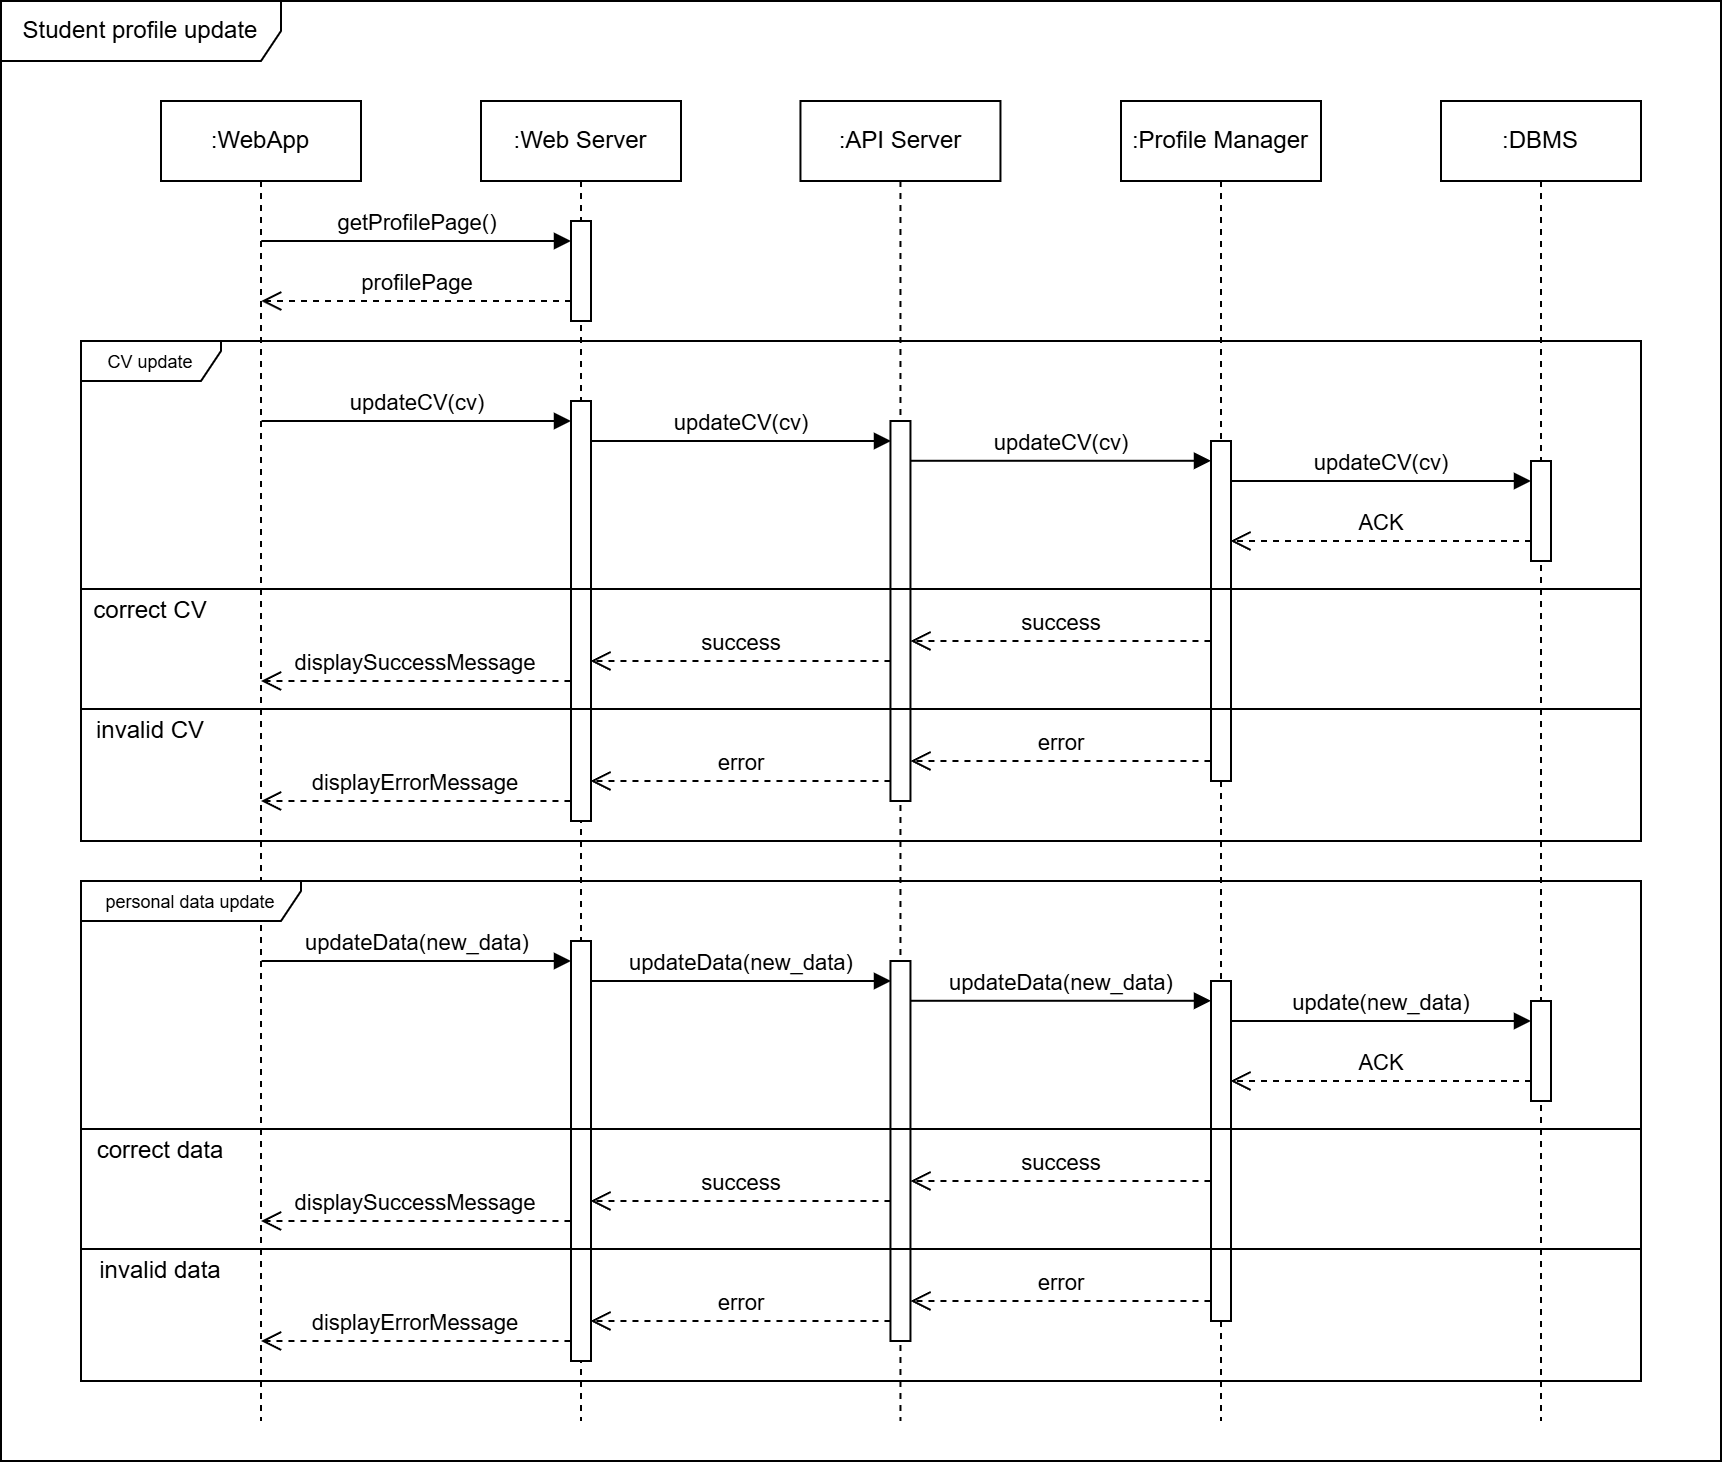
\includegraphics[width=1\linewidth]{Images/Sequence diagrams/UC4.png}
        \caption{Student's Profile Update}
        \label{fig:enter-label}
    \end{figure}
\end{center}

\textbf{UC\cuc\ - UC\cuc\ - UC\cuc\  - Student checks available offers, opens the details page of an internship post, and sends an application for it} \\
The diagram shows the application process for internships. The WebApp requests internship details through the Web Server, which retrieves them via the API Server from the Internship Manager and DBMS. After reviewing, the student sends an application, which is processed and stored. Feedback on success or errors is then displayed to the student.
\begin{center}
    \begin{figure}[H]
        \centering
        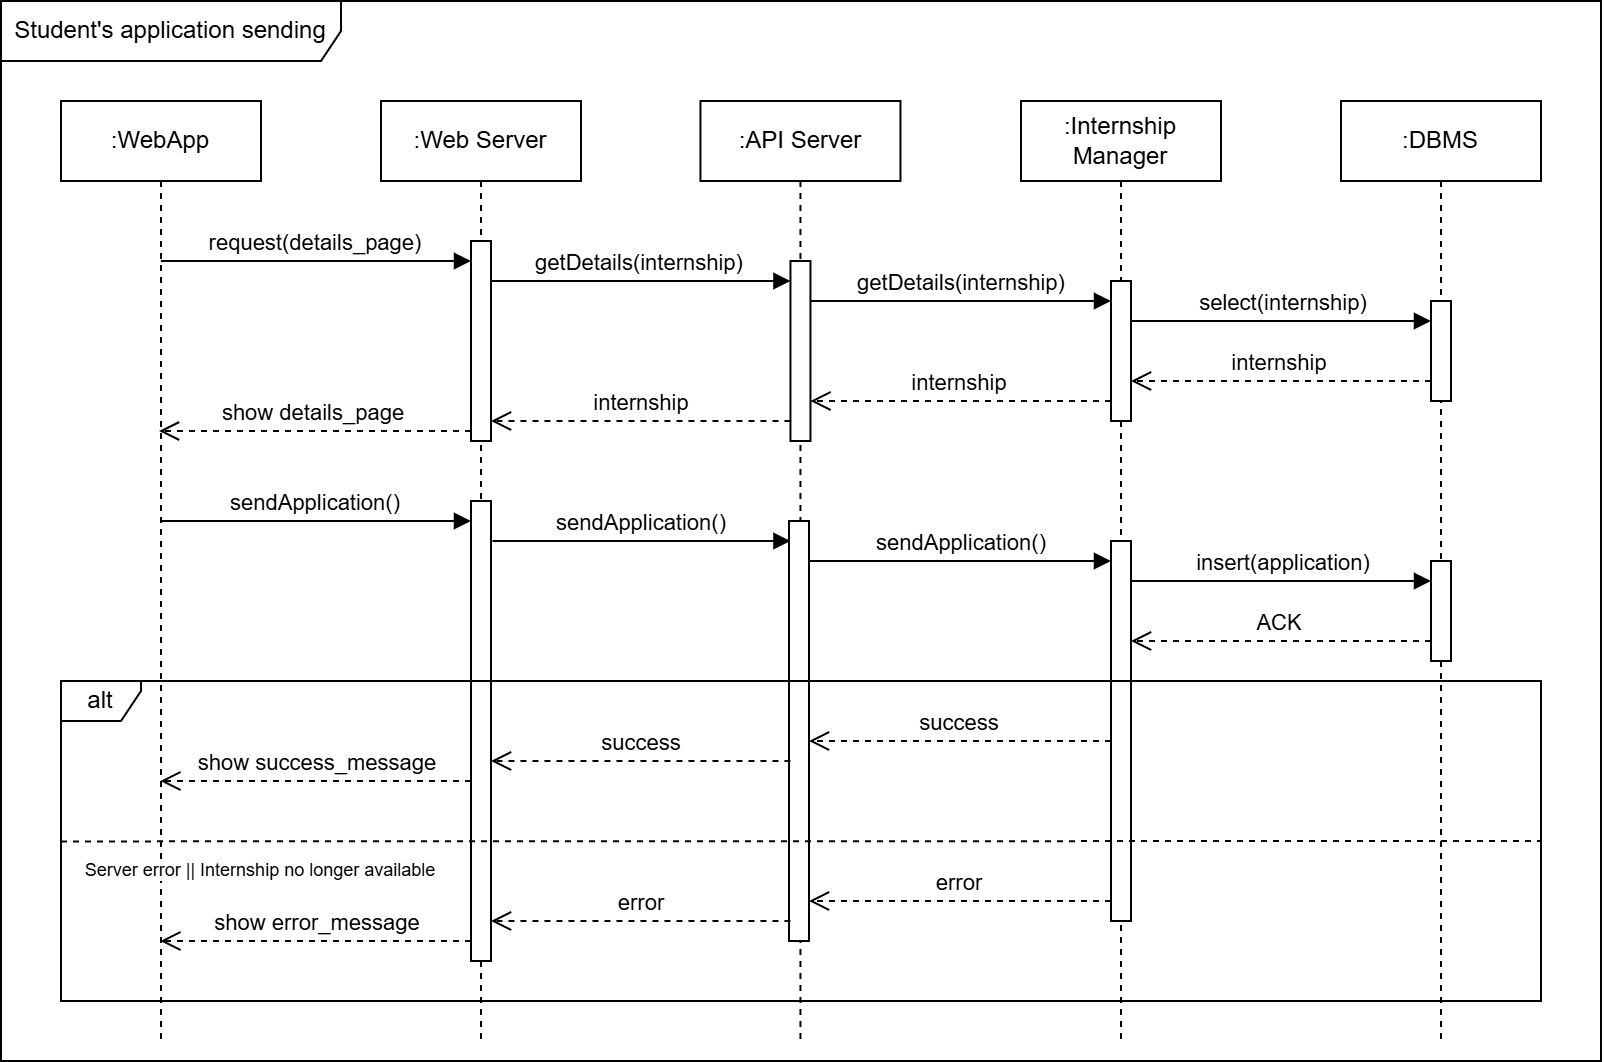
\includegraphics[width=1\linewidth]{Images/Sequence diagrams/UC567.png}
        \caption{Student's Application sending Update}
        \label{fig:enter-label}
    \end{figure}
\end{center}

\textbf{UC\cuc\ - Student accepts or denies an interview schedule proposal from the company} \\
The diagram illustrates the process for a student's schedule response. Notifications are sent from the Internship Manager through the API Server to the WebApp. The student can either accept or reject the schedule. The respective action triggers an action, processed by the Internship Manager and reflected in the DBMS. A confirmation message is then displayed to the student on the WebApp.
\begin{center}
    \begin{figure}[H]
        \centering
        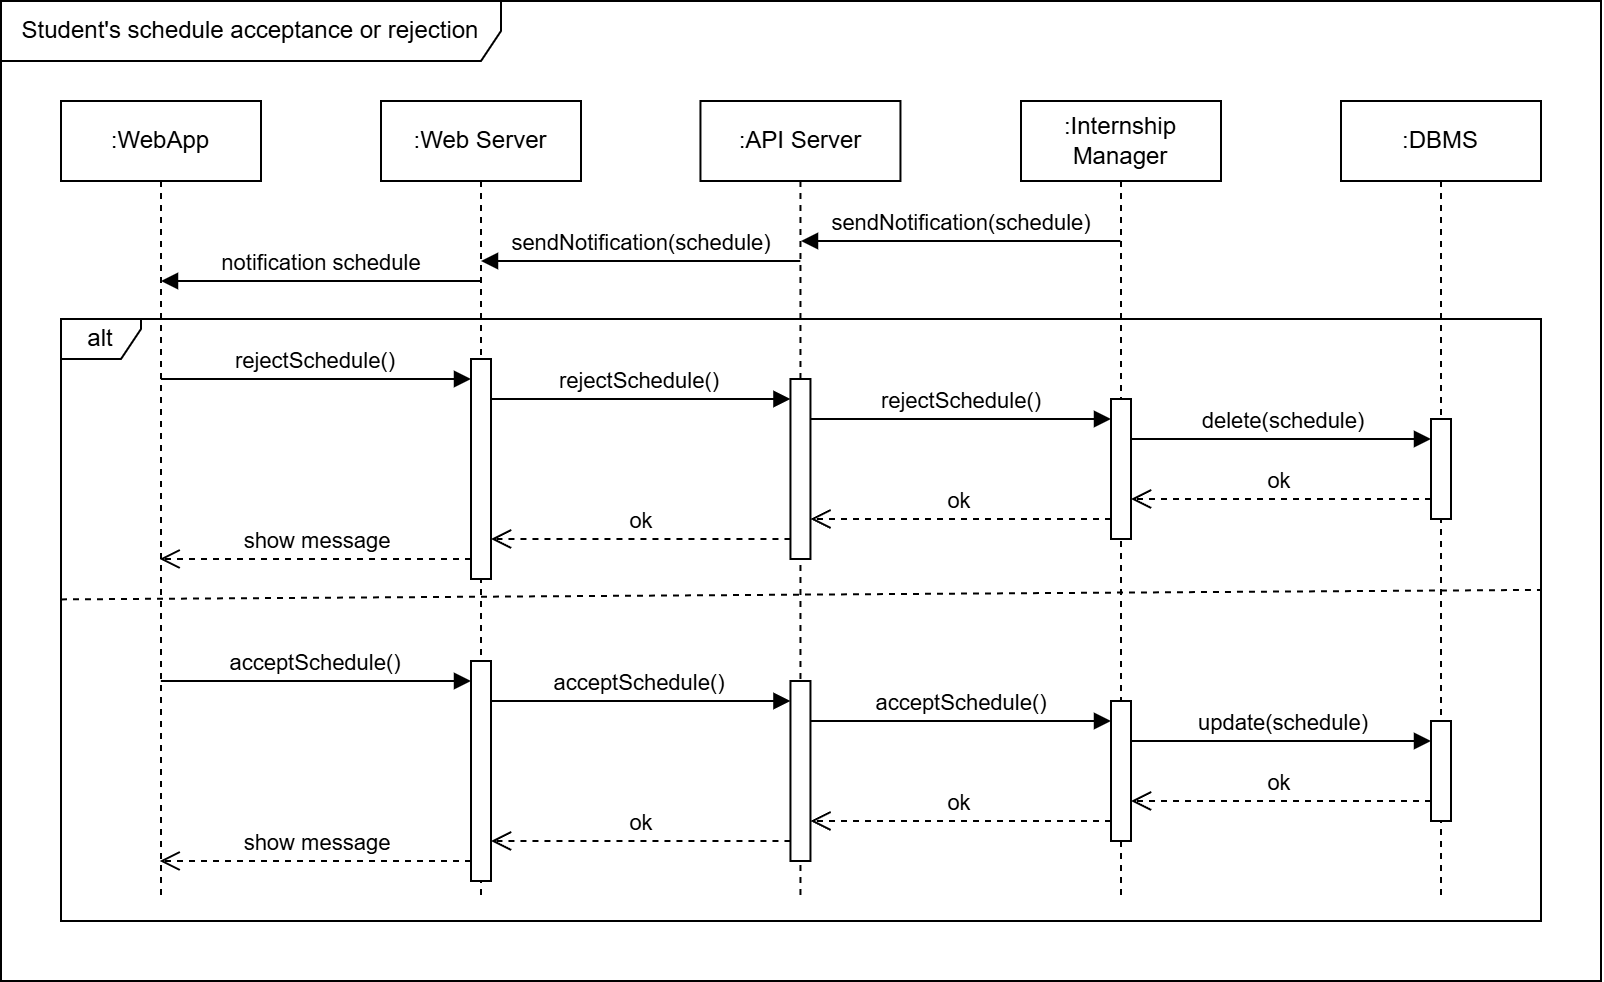
\includegraphics[width=1\linewidth]{Images/Sequence diagrams/UC8.png}
        \caption{Student's Application sending Update}
        \label{fig:enter-label}
    \end{figure}
\end{center}

\textbf{UC\cuc\ - Student accepts or denies the start of the internship} \\
The diagram illustrates the process for the final decision of a student. The student receives a notification to confirm or reject the start of the internship, following the positive decision of the company after the interview. If the student accepts, the confirmation is sent through the Web Server and API Server to the Internship Manager, which updates the database to finalize the start. If the student rejects, a similar process is followed to record the rejection in the database. In both scenarios, a success message is displayed.
\begin{center}
    \begin{figure}[H]
        \centering
        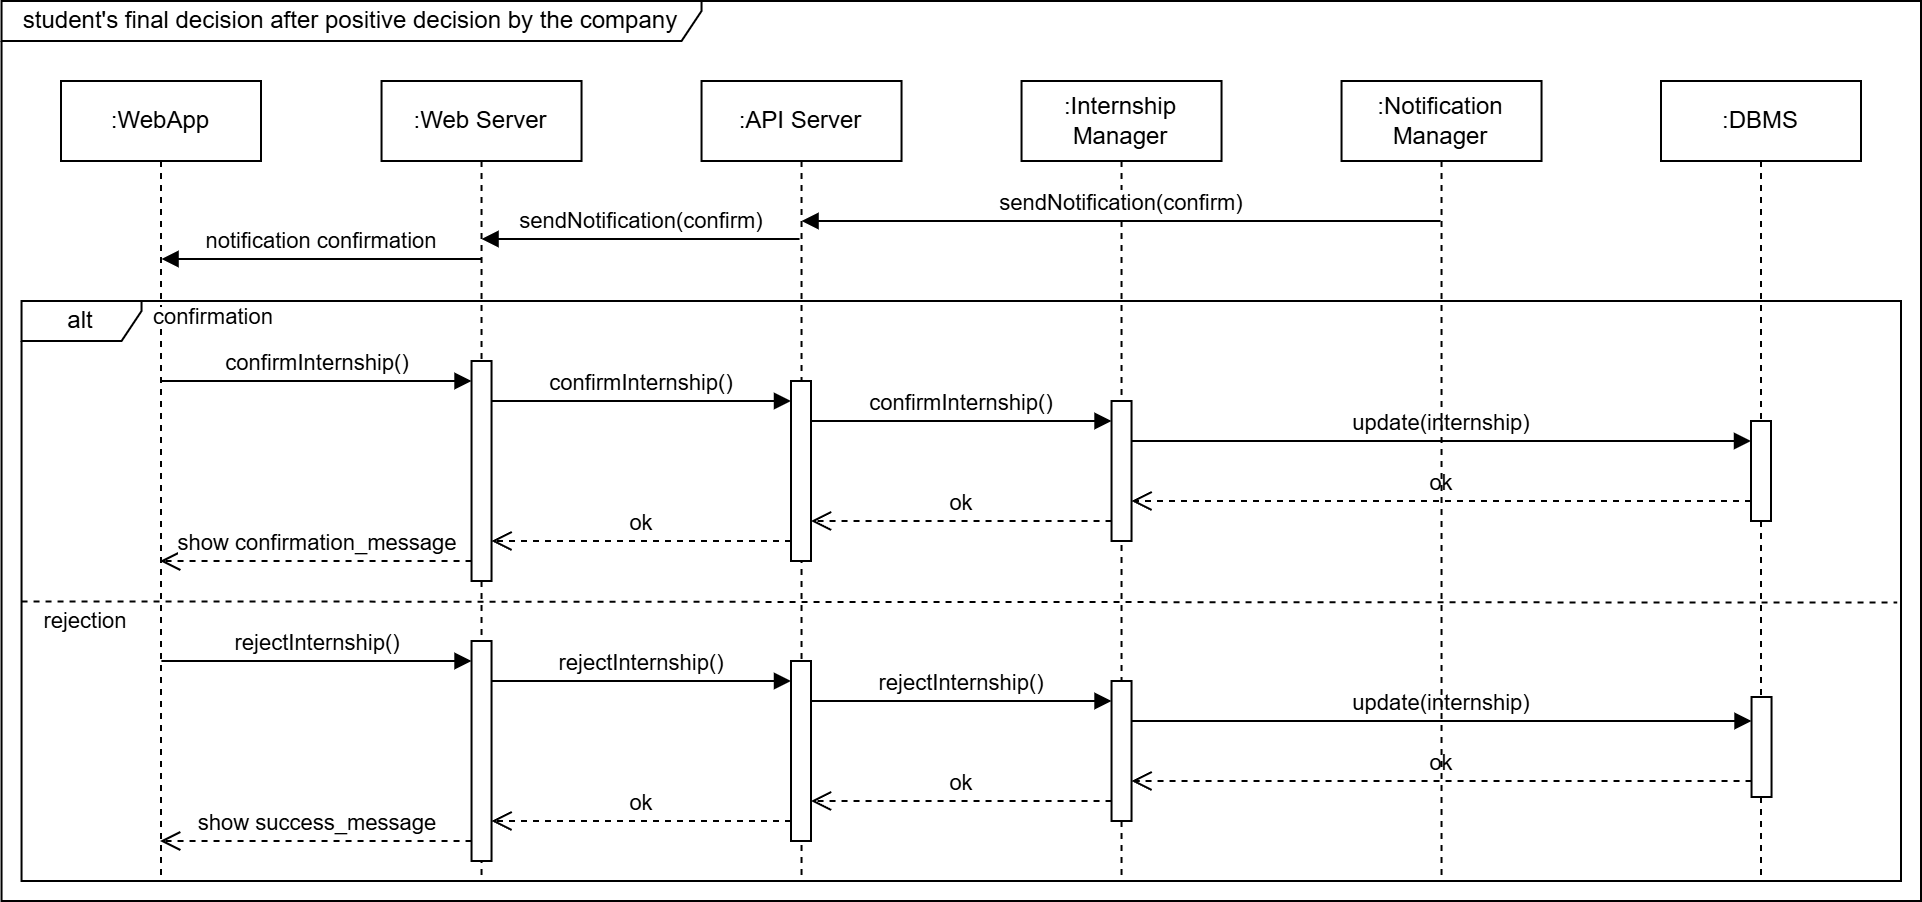
\includegraphics[width=1\linewidth]{Images/Sequence diagrams/UC9.png}
        \caption{Student's Application sending Update}
        \label{fig:enter-label}
    \end{figure}
\end{center}

\textbf{UC\cuc\  - Company’s account activation} \\
The figure shows the process of upgrading an account from standard registered user to a verified company account. The process consists of inserting the additional details required to do the upgrade correctly and checking that there are no other companies with the same credentials.
\begin{center}
    \begin{figure}[H]
        \centering
        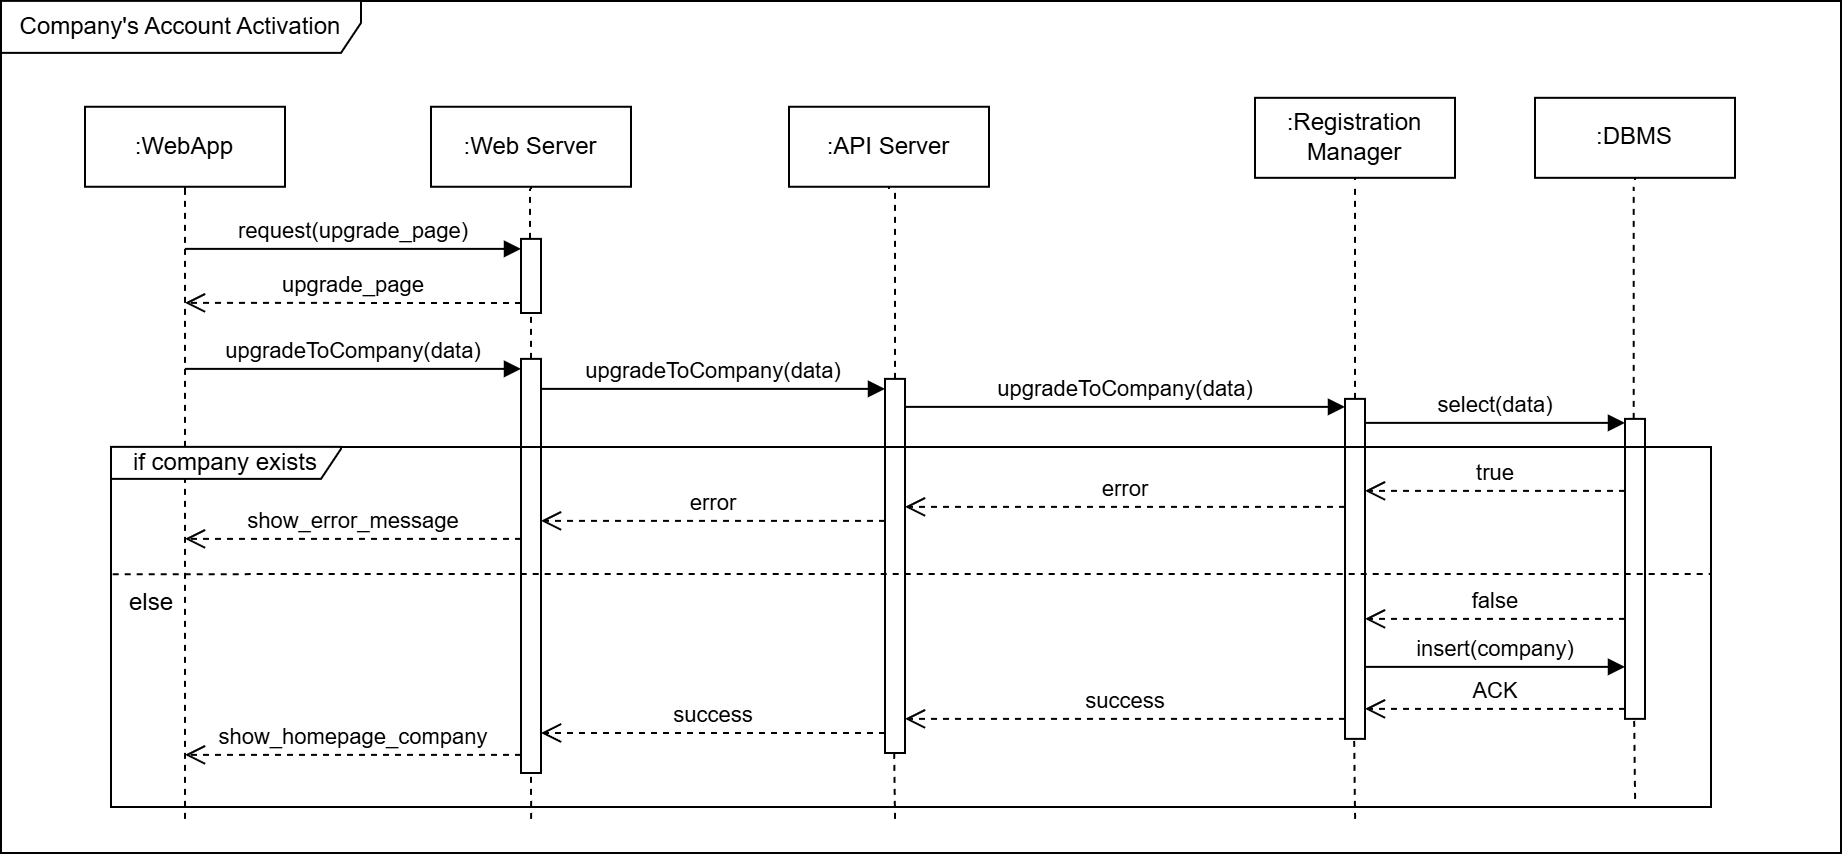
\includegraphics[width=1\linewidth]{Images/Sequence diagrams/UC10.png}
        \caption{Company Account Activation}
        \label{fig:enter-label}
    \end{figure}
\end{center}

\textbf{UC\cuc\  - Company's profile modification} \\
The diagram shows the process for updating a company's profile. The company accesses its profile page to modify its information. After making the desired changes, the updated data are sent through the Web Server and API Server to the Profile Manager. The Profile Manager validates the modifications and updates the database. In case of a successful completion, a confirmation message is displayed to the company. In case of errors, an error message is shown instead.
\begin{center}
    \begin{figure}[H]
        \centering
        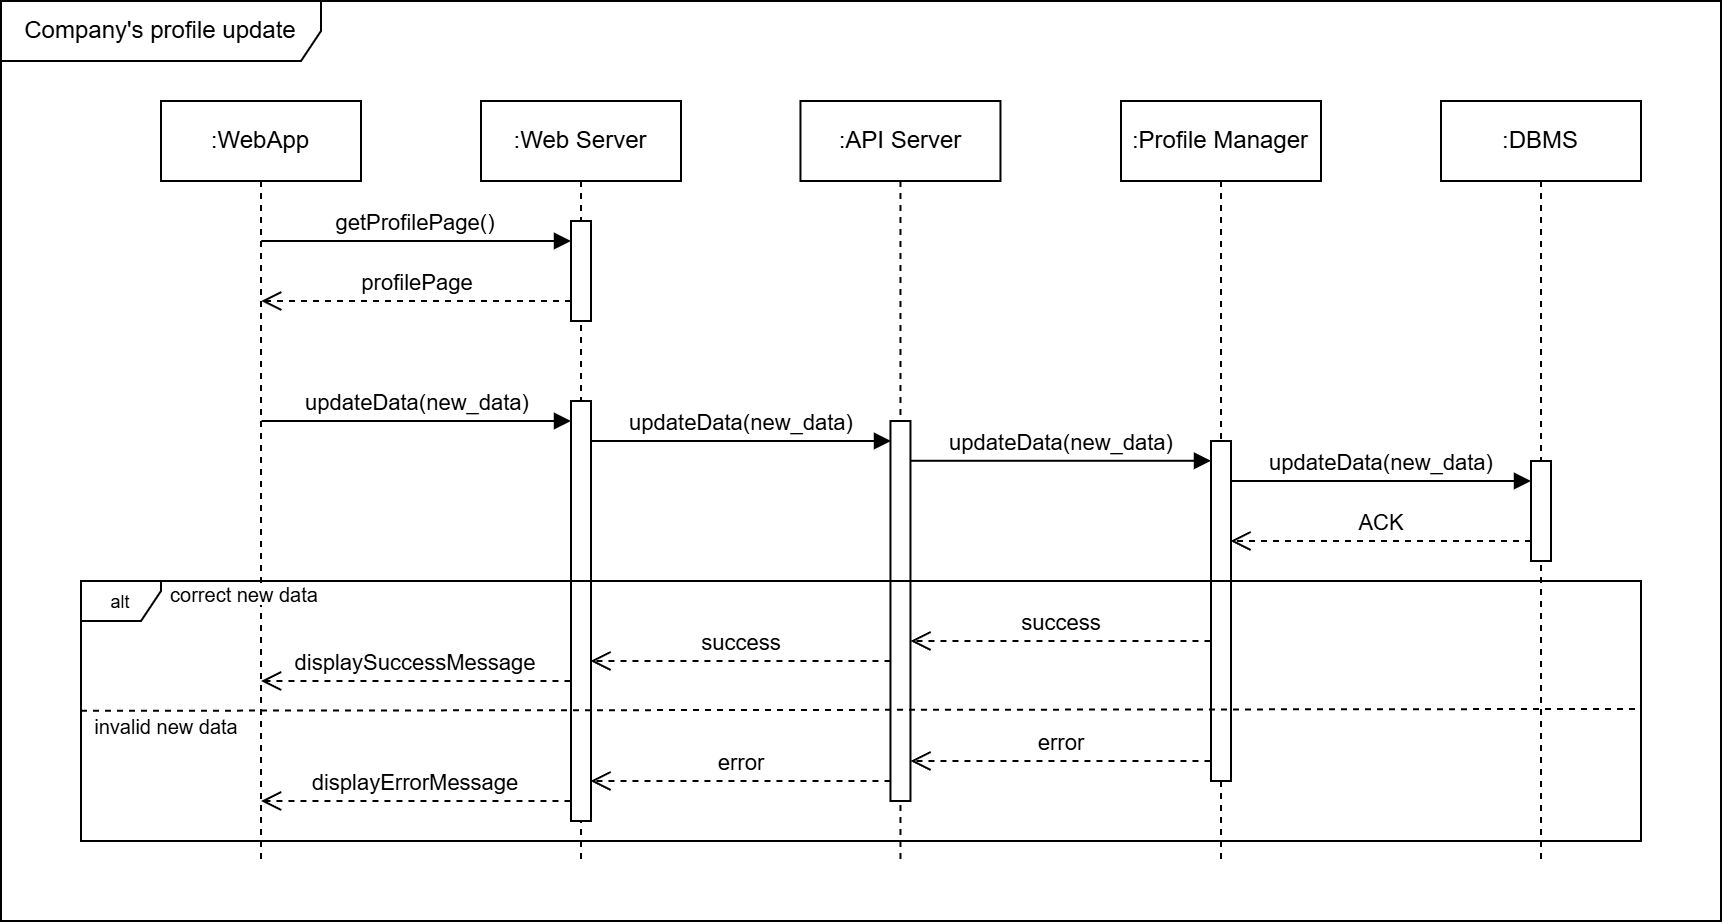
\includegraphics[width=1\linewidth]{Images/Sequence diagrams/UC11.png}
        \caption{Company's Profile Update}
        \label{fig:enter-label}
    \end{figure}
\end{center}

\textbf{UC\cuc\ - Company posts a new internship} \ The figure shows the process of posting a new internship offer by a company. The company accesses the dedicated page with a form, fills in all the fields, and submits the required data. After the request is submitted to the Web Server and API Server, it is forwarded to the Internship Manager. The Internship Manager validates the data and proceeds to insert it into the database. In case of successful completion, a confirmation message is displayed to the company. In case of errors, an error message is shown instead.
\begin{center}
    \begin{figure}[H]
        \centering
        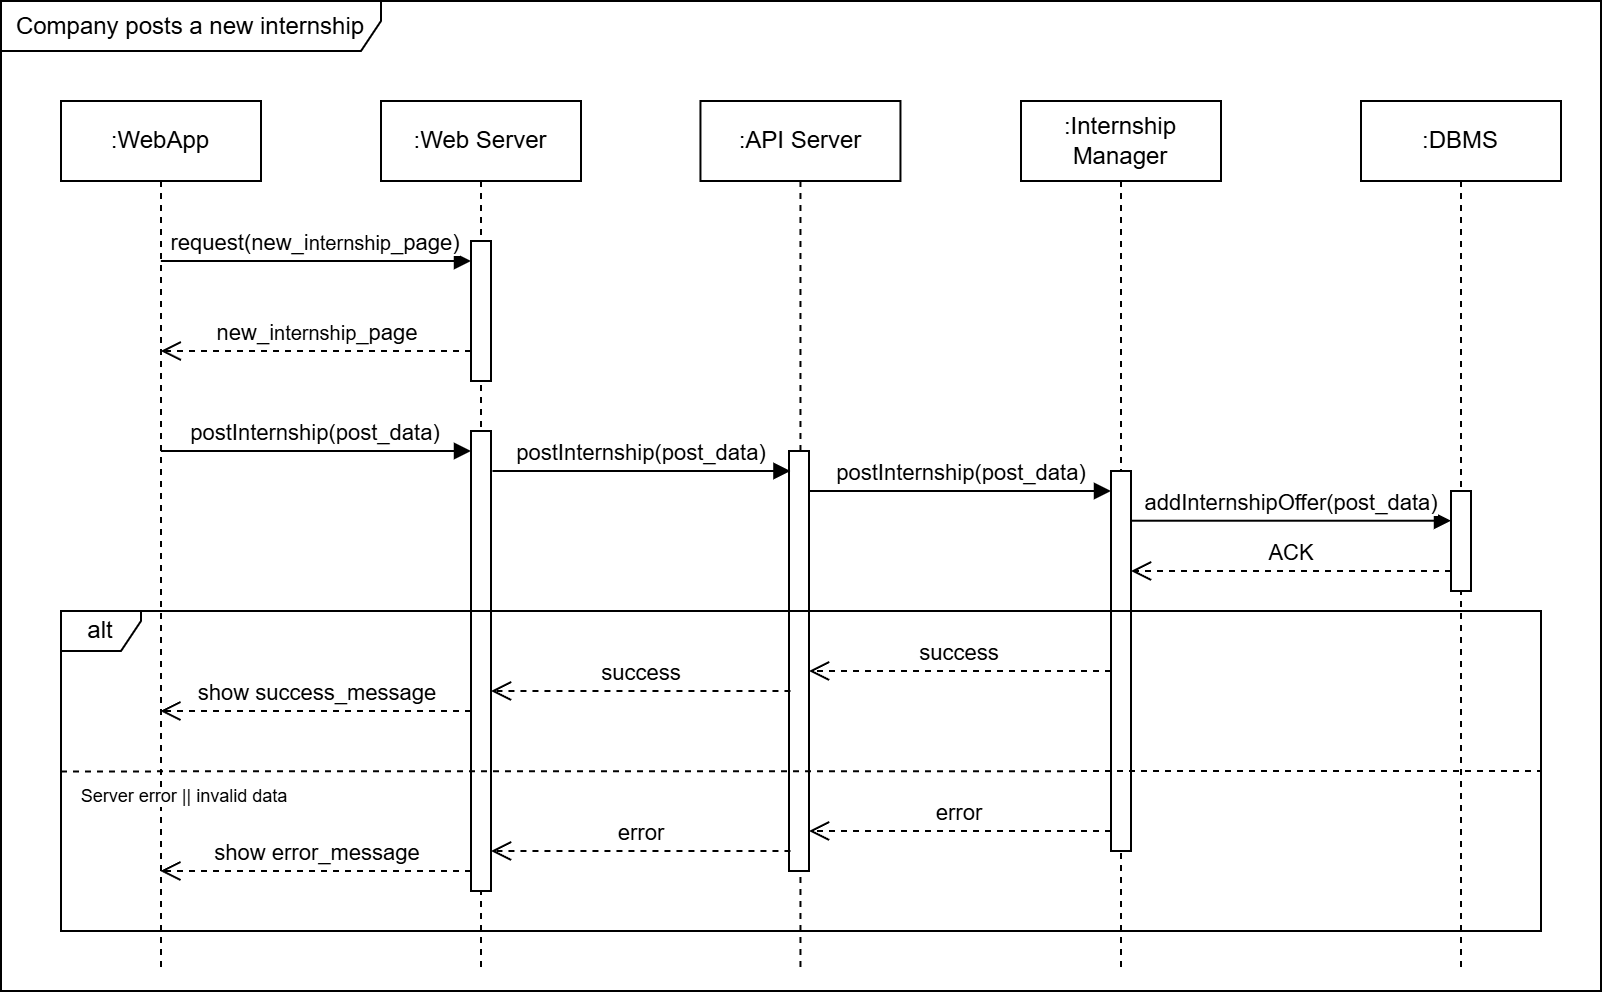
\includegraphics[width=1\linewidth]{Images/Sequence diagrams/UC12.png}
        \caption{Company new offer posting}
        \label{fig:enter-label}
    \end{figure}
\end{center}

\textbf{UC\cuc\  - The company accepts an application or identifies a promising student and
proposes a schedule for the interview} \\
The diagram illustrates the process where a company selects candidates for an internship, views a student's details, and proposes a schedule. The WebApp communicates with the Web Server, API Server, and respective managers (Matchmaking, Profile, Internship) to retrieve data and submit the schedule. Success or error messages are displayed based on the operation outcome.
\begin{center}
    \begin{figure}[H]
        \centering
        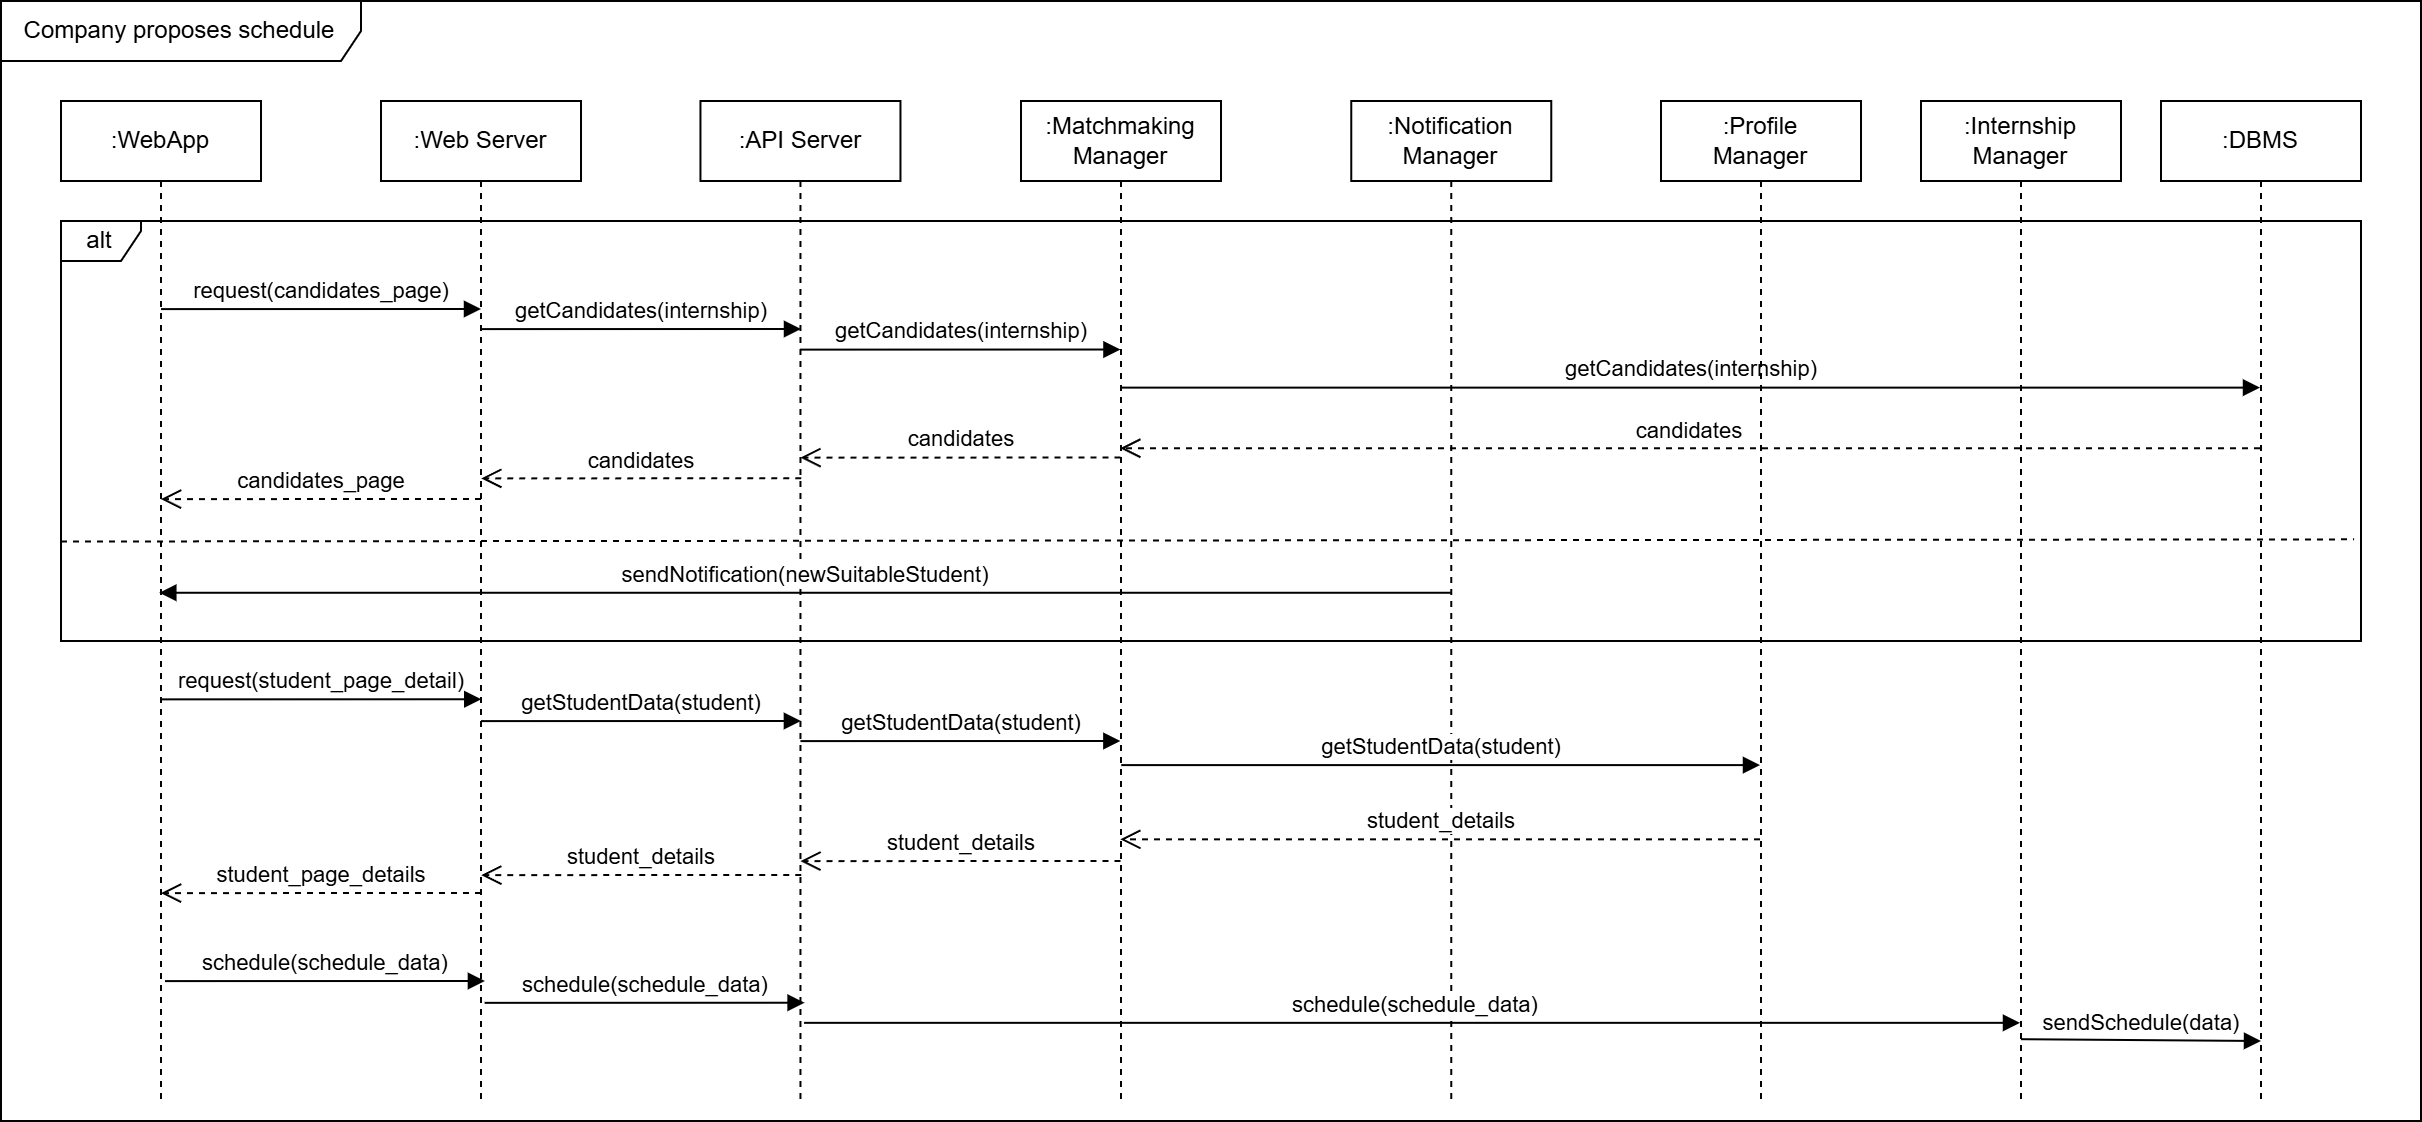
\includegraphics[width=1\linewidth]{Images/Sequence diagrams/UC13.png}
        \caption{Company schedule interview}
        \label{fig:enter-label}
    \end{figure}
\end{center}

\textbf{UC\cuc\  - Student or Company submits a complaint about an ongoing internship} \\
The figure shows the process of submitting a new complaint on an internship by a student or a company. The student or company submits it through the platform. The complaint is sent via the Web Server and API Server to the Complaint Manager, which logs the issue in the database. After the complaint is recorded, the Complaint Manager sends a notification through the Notification Manager to the student’s university to alert them about the new complaint. The system then confirms the submission with a success message or informs the user of any errors encountered during the process.
\begin{center}
    \begin{figure}[H]
        \centering
        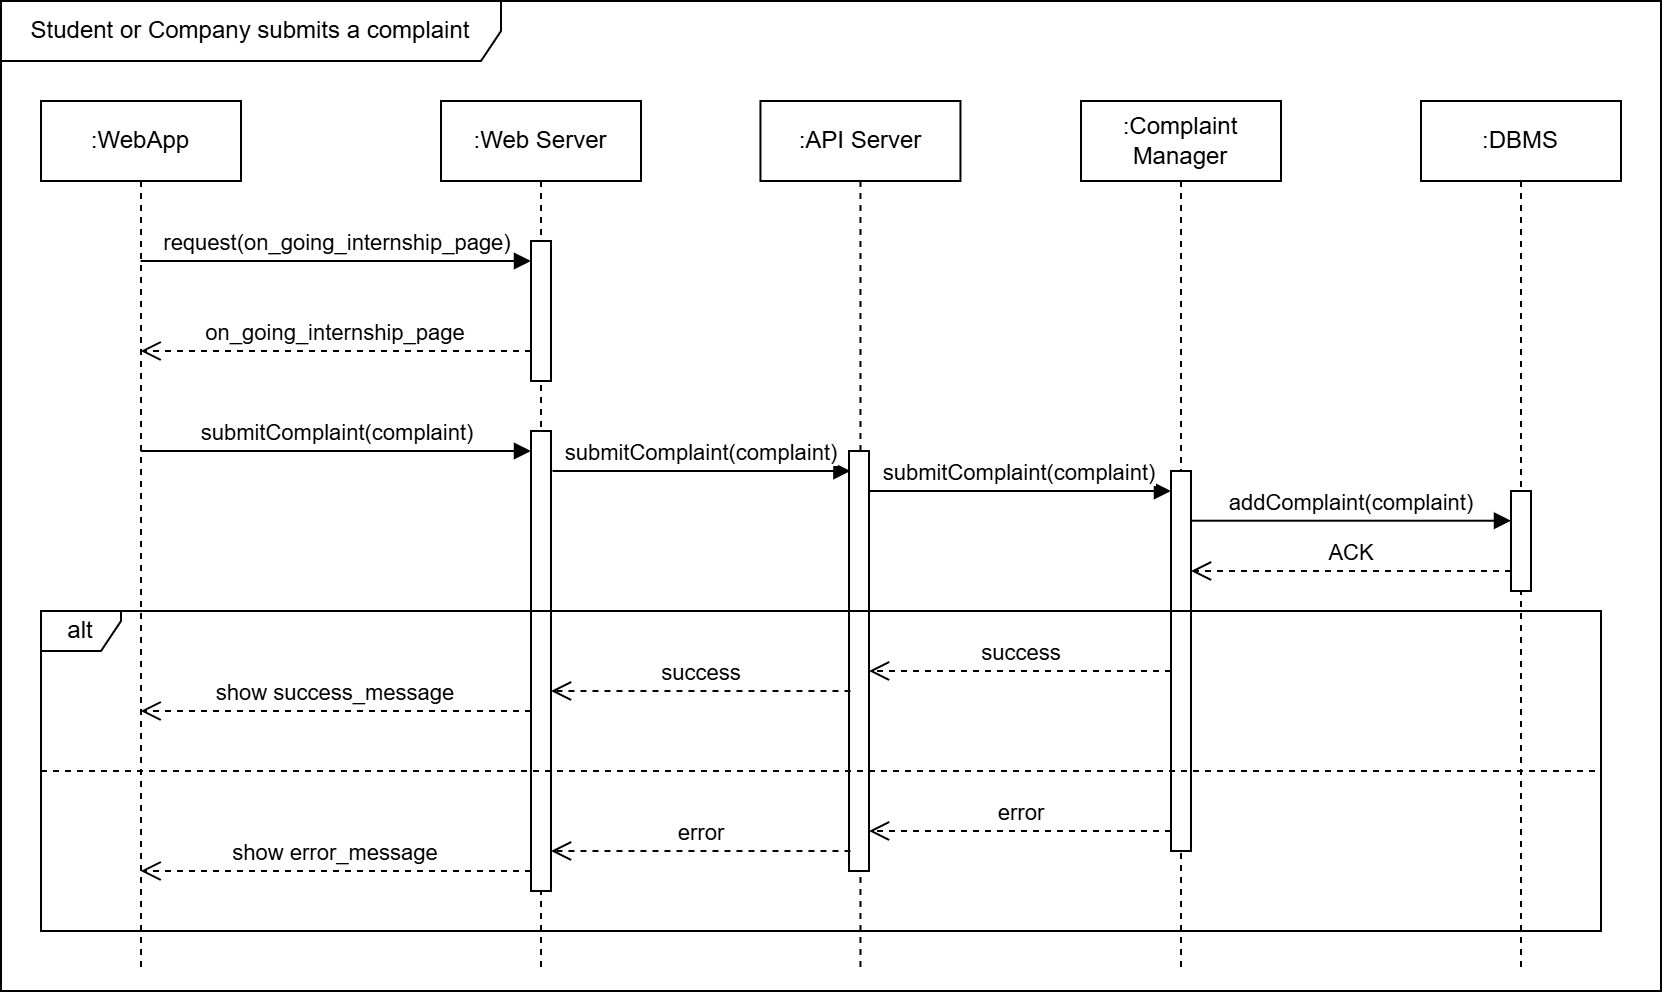
\includegraphics[width=1\linewidth]{Images/Sequence diagrams/UC14.png}
        \caption{Company new offer posting}
        \label{fig:enter-label}
    \end{figure}
\end{center}

\textbf{UC\cuc\  - Student or Company submits a feedback about a terminated internship} \\
The figure shows the process of submitting a feedback on a terminated internship by a student or a company. The student or company submits it through the platform. The feedback is processed via the Web Server and API Server and stored in the database by the Feedback Manager. After successfully recording the feedback, the system confirms the submission with a success message or informs the user of any errors. Additionally, the Feedback will be used for future analysis and reference.
\begin{center}
    \begin{figure}[H]
        \centering
        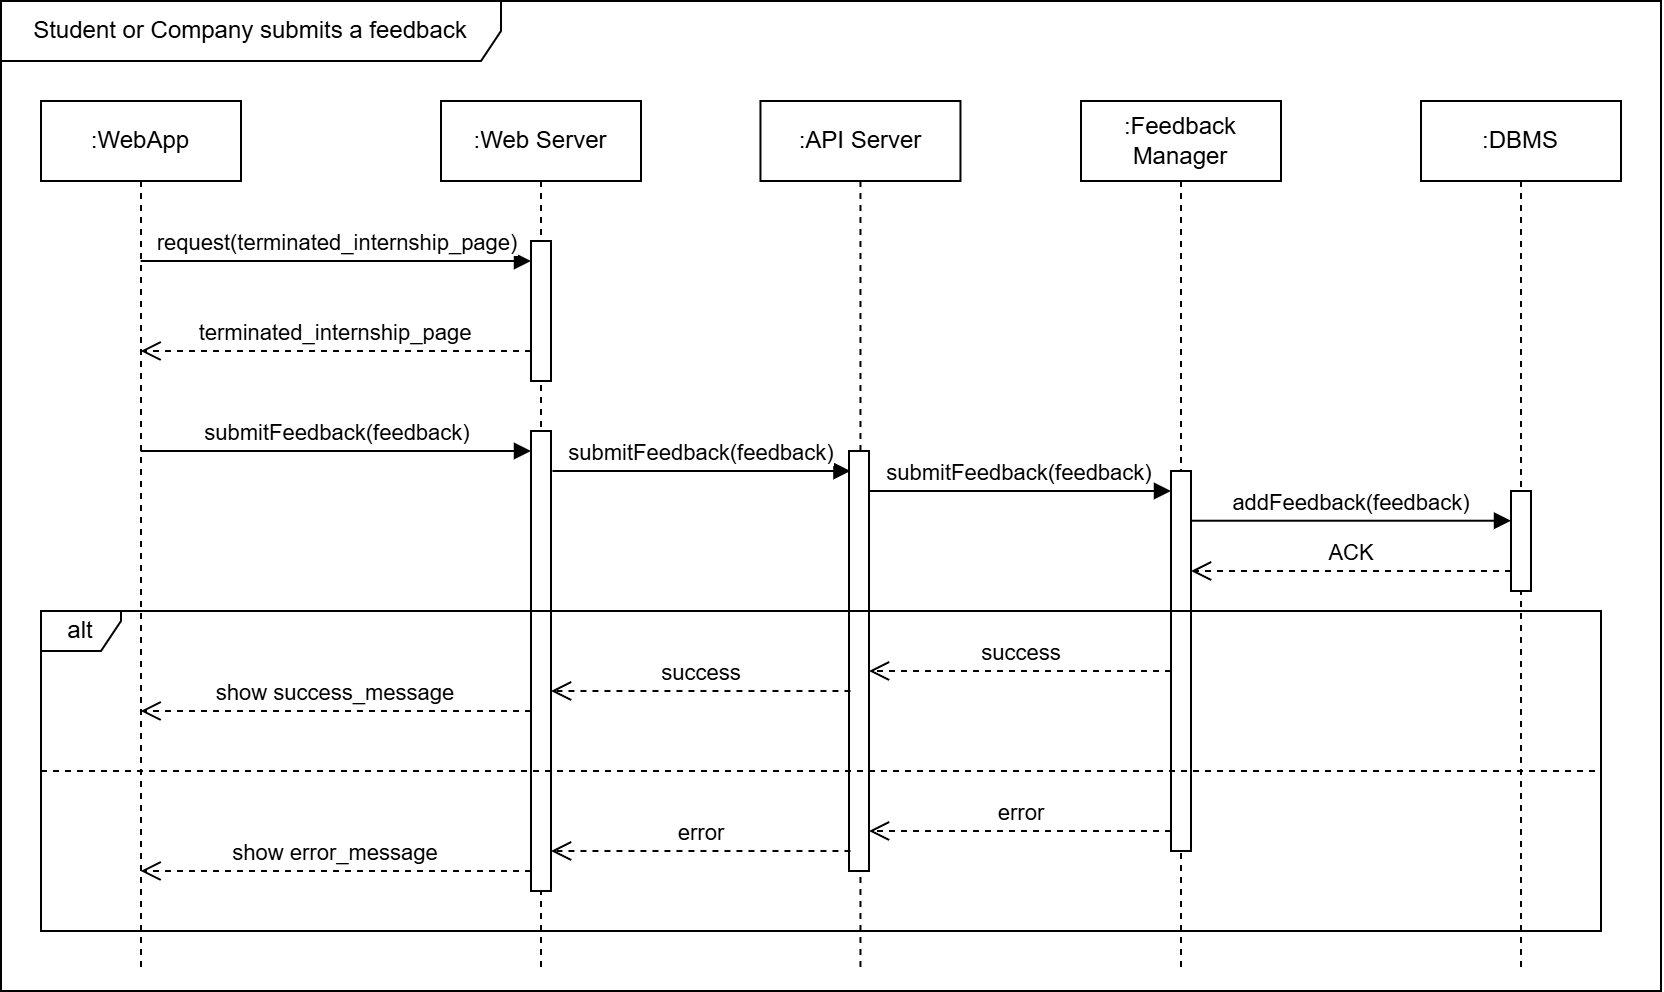
\includegraphics[width=1\linewidth]{Images/Sequence diagrams/UC15.png}
        \caption{Company new offer posting}
        \label{fig:enter-label}
    \end{figure}
\end{center}

\textbf{UC\cuc\  - University decides to interrupt an internship due to relevant complaints} \\
The figure shows the process of interrupting an internship. The university reviews relevant complaints about an ongoing internship and decides to interrupt it. The decision is submitted through the platform and processed via the Web Server and API Server. The Internship Manager updates the database to mark the internship as interrupted and notifies both the company and the student about the decision. A confirmation message is displayed to the university upon successful completion.
\begin{center}
    \begin{figure}[H]
        \centering
        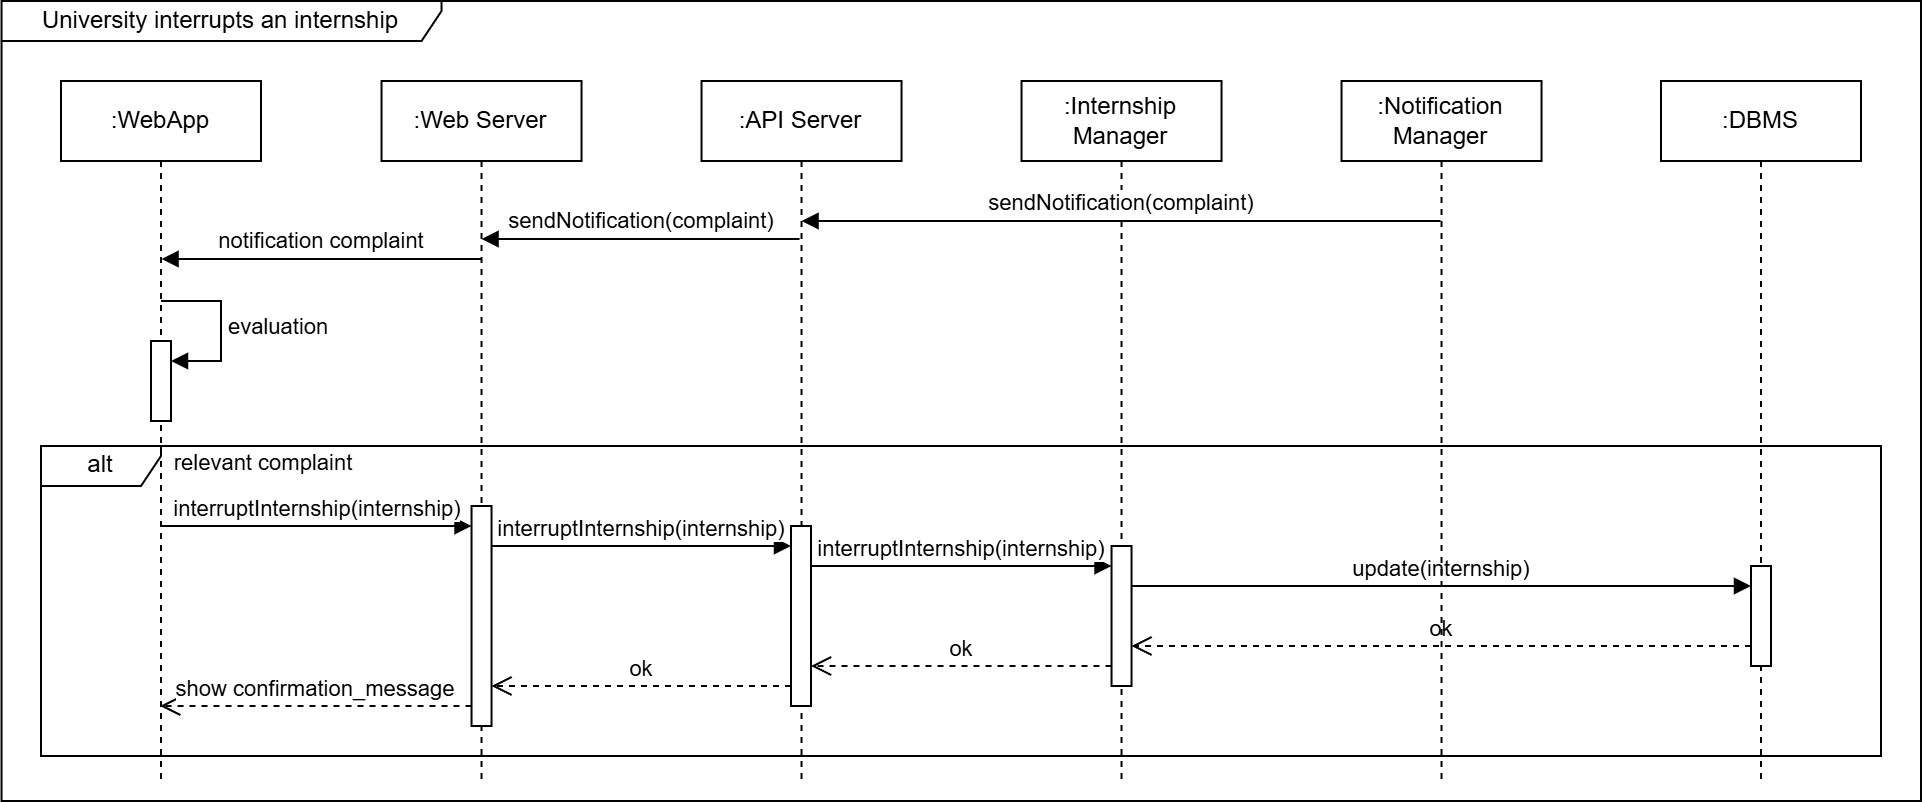
\includegraphics[width=1\linewidth]{Images/Sequence diagrams/UC16.png}
        \caption{Company new offer posting}
        \label{fig:enter-label}
    \end{figure}
\end{center}

% Add runtime view details here.

\section{Component Interfaces}
\label{sec:component_interfaces}
\textbf{Login manager}
\begin{itemize}
    \item \textit{login(String username, String password): boolean}
\end{itemize}
\textbf{Registration manager}
\begin{itemize}
\item \textit{register(String name, String surname, String email) : Boolean}
    \item \textit{upgradeToStudentAccount(User user, String name, String surname, String academicEmail, String phoneNumber, String postalCode, File CV, List<String> goals): boolean}
    \item u\textit{pgradeToCompanyAccount(User user, String fullName, String phoneNumber, String officeAddress): boolean}
\end{itemize}
\textbf{Profile manager}
\begin{itemize}
    \item \textit{getStudentData(Student student): Student}
    \item \textit{updateStudentData(Student student, String name, String surname, String academicEmail, String phoneNumber, String postalCode, List<String> goals): boolean}
    \item \textit{updateStudentCV(Student student, File CV): boolean}
    \item \textit{getCompanyData(Company company): Company}
    \item \textit{updateCompanyData(Company company, String fullName, String phoneNumber, String officeAddress): boolean}
\end{itemize}
\textbf{Internship manager}
\begin{itemize}
    \item \textit{addInternshipOffer(Company company, String projectDescription, String role, String address, Float salary, Int numberOfStudents, List<String> skills, String weeklySchedule, List<String> benefits): boolean}
    \item \textit{updateInternshipOffer(Internship internship, String projectDescription, String role, String address, Float salary, Int numberOfStudents, List<String> skills, String weeklySchedule, List<String> benefits): boolean}
    \item \textit{deleteInternshipOffer(Internship internship): boolean}
    \item \textit{acceptApplication(Application application): boolean}
    \item \textit{sendSchedule(Internship internship, Student student, String schedule): boolean}
    \item \textit{rejectApplication(Application application): boolean}
    \item \textit{confirmInternship(Internship internship, Student student): boolean}
    \item \textit{rejectInternship(Internship internship, Student student): boolean}
\end{itemize}
\textbf{Matchmaking manager}
\begin{itemize}
    \item \textit{generateRecommendationsForStudent(Student student): List<Internship>}
    \item \textit{generateRecommendationsForStudent(Internship internship): List<Student>}
    \item \textit{findBestMatch(Student student): Internship}
    \item \textit{findBestMatch(Internship internship): Student}
    \item \textit{getCandidates(Internship internship): List<Student>}
\end{itemize}
\textbf{Complaint manager}
\begin{itemize}
    \item \textit{submitComplaint(Internship internship, Student student, String complaintText): boolean}
    \item \textit{submitComplaint(Internship internship, Company company, String complaintText): boolean}
    \item \textit{getComplaintStatus(Complaint complaint): ComplaintStatus}
    \item \textit{getCompliantsByInternship(Internship internship): List<Complaint>}
    \item \textit{interruptInternship(Internship internship, String reason): boolean}
\end{itemize}
\textbf{Feedback manager}
\begin{itemize}
    \item \textit{submitFeedback(Internship internship, Student student, String feedbackText): boolean}
    \item \textit{submitFeedback(Internship internship, Company company, String feedbackText): boolean}
    \item \textit{getFeedbackByInternship(Internship internship): List<Feedback>}
    \item \textit{analyzeFeedback(Feedback feedback): boolean}
\end{itemize}
\textbf{Notification manager}
\begin{itemize}
    \item \textit{sendNotification(User user, NotificationType type, String message): boolean}
    \item \textit{getNotifications(User user): List<Notification>}
\end{itemize}

% Describe the component interfaces here.

\section{Selected Architectural Styles and Patterns}
\label{sec:architectural_styles_patterns}
\subsection{3-tiered Architecture}
The architectural style chosen is 3-tiered architecture, which provides significant benefits such as modularization into three distinct layers:
\begin{itemize}
    \item Web and Mobile Client : This is the presentation tier and gives access to the user interface. The web application provides the user interface through a browser, utilizing technologies like HTML, CSS, and JavaScript for dynamic and interactive content. The mobile application delivers a native or hybrid experience, optimized for smaller screens and supporting additional functionalities like push notifications.
    \item The S\&C API server : This is the middle tier, responsible for implementing the business logic of the system. It handles tasks such as user authentication, internship matching, and processing of user actions. The application server communicates with the database server and ensures the seamless operation of system workflows.
    \item The database server : This is the backend of the application, powered by a Database Management System (DBMS) like MySQL. It stores and manages all system data, including user profiles, internship postings, applications, complaints and feedback, ensuring data integrity and quick retrieval for the application server.
\end{itemize}
% Add information about architectural styles and patterns here.

\section{Other Design Decisions}
\label{sec:other_design_decisions}
This section is focused on explaining the design decisions  that have been implemented in order to make the system work correctly.
\subsection{Availability}
Load balancing is implemented to create a system with a high availability and capable of handling a large amount of concurrent requests efficiently. In addition to this, it is crucial to incorporate replication mechanism in order to eliminate single points of failure and enhance system reliability.
\subsection{Data Storage}
Data storage is managed through the use of a database to store the personal information of users, students, universities and companies. Additionally, auxiliary data structures are used in order to make query performance better. 